%%
%% MCUlab (c) 2021-22 Christopher A. Bohn
%%
%% Licensed under the Apache License, Version 2.0 (the "License");
%% you may not use this file except in compliance with the License.
%% You may obtain a copy of the License at
%%     http://www.apache.org/licenses/LICENSE-2.0
%% Unless required by applicable law or agreed to in writing, software
%% distributed under the License is distributed on an "AS IS" BASIS,
%% WITHOUT WARRANTIES OR CONDITIONS OF ANY KIND, either express or implied.
%% See the License for the specific language governing permissions and
%% limitations under the License.
%%

%%
%% (c) 2021 Christopher A. Bohn
%%

\documentclass[12pt]{article}

\usepackage{fullpage}
\usepackage{fancyhdr}
\usepackage[procnames]{listings}
\usepackage{hyperref}
\usepackage{textcomp}
\usepackage{bold-extra}
\usepackage[dvipsnames]{xcolor}
\usepackage{etoolbox}


% Customize the semester (or quarter) and the course number

\newcommand{\courseterm}{Spring 2022}
\newcommand{\coursenumber}{CSCE 231}

% Customize how a typical lab will be managed;
% you can always use \renewcommand for one-offs

\newcommand{\runtimeenvironment}{your account on the \textit{csce.unl.edu} Linux server}
\newcommand{\filesource}{Canvas or {\footnotesize$\sim$}cse231 on \textit{csce.unl.edu}}
\newcommand{\filesubmission}{Canvas}

% These are placeholder commands and will be renewed in each lab

\newcommand{\labnumber}{}
\newcommand{\labname}{Lab \labnumber\ Assignment}
\newcommand{\shortlabname}{}
\newcommand{\duedate}{}

% Individual or team effort

\newcommand{\individualeffort}{This is an individual-effort project. You may discuss concepts and syntax with other students, but you may discuss solutions only with the professor and the TAs. Sharing code with or copying code from another student or the internet is prohibited.}
\newcommand{\teameffort}{This is a team-effort project. You may discuss concepts and syntax with other students, but you may discuss solutions only with your assigned partner(s), the professor, and the TAs. Sharing code with or copying code from a student who is not on your team, or from the internet, is prohibited.}
\newcommand{\freecollaboration}{In addition to the professor and the TAs, you may freely seek help on this assignment from other students.}
\newcommand{\collaborationrules}{}

% Do you care about software engineering?

\providebool{allowspaghetticode}

\setbool{allowspaghetticode}{false}

\newcommand{\softwareengineeringfrontmatter}{
    \ifboolexpe{not bool{allowspaghetticode}}{
        \section*{No Spaghetti Code Allowed}
        In the interest of keeping your code readable, you may \textit{not} use
        any \lstinline{goto} statements, nor may you use any \lstinline{break}
        statements to exit from a loop, nor may you have any functions
        \lstinline{return} from within a loop.
    }{}
}

\newcommand{\spaghetticodepenalties}[1]{
    \ifboolexpe{not bool{allowspaghetticode}}{
        \penaltyitem{1}{for each \lstinline{goto} statement, \lstinline{break}
            statement used to exit from a loop, or \lstinline{return} statement
            that occurs within a loop.}
    }{}
}

% You shouldn't need to customize these,
% but you can if you like

\lstset{language=C, tabsize=4, upquote=true, basicstyle=\ttfamily}
\newcommand{\function}[1]{\textbf{\lstinline{#1}}}
\setlength{\headsep}{0.7cm}
\hypersetup{colorlinks=true}

\newcommand{\startdocument}{
    \pagestyle{fancy}
    \fancyhf{}
    \lhead{\coursenumber}
    \chead{\ Lab \labnumber: \labname}
    \rhead{\courseterm}
    \cfoot{\shortlabname-\thepage}

	\begin{document}
	\title{\ Lab \labnumber}
	\author{\labname}
	\date{Due: \duedate}
	\maketitle

    \textit{\collaborationrules}
}

\newcommand{\rubricitem}[2]{\item[\underline{\hspace{1cm}} +#1] #2}
\newcommand{\bonusitem}[2]{\item[\underline{\hspace{1cm}} Bonus +#1] #2}
\newcommand{\penaltyitem}[2]{\item[\underline{\hspace{1cm}} -#1] #2}

%%
%% labs/common/semester.tex
%% (c) 2021-22 Christopher A. Bohn
%%
%% Licensed under the Apache License, Version 2.0 (the "License");
%% you may not use this file except in compliance with the License.
%% You may obtain a copy of the License at
%%     http://www.apache.org/licenses/LICENSE-2.0
%% Unless required by applicable law or agreed to in writing, software
%% distributed under the License is distributed on an "AS IS" BASIS,
%% WITHOUT WARRANTIES OR CONDITIONS OF ANY KIND, either express or implied.
%% See the License for the specific language governing permissions and
%% limitations under the License.
%%


% Customize the semester (or quarter) and the course number

\newcommand{\courseterm}{Fall 2022}
\newcommand{\coursenumber}{CSCE 231}

% Customize how a typical lab will be managed;
% you can always use \renewcommand for one-offs

\newcommand{\runtimeenvironment}{your account on the \textit{csce.unl.edu} Linux server}
\newcommand{\filesource}{Canvas or {\footnotesize$\sim$}cse231 on \textit{csce.unl.edu}}
\newcommand{\filesubmission}{Canvas}

% Customize for the I/O lab hardware

\newcommand{\developmentboard}{Arduino Nano}
%\newcommand{\serialprotocol}{SPI}
\newcommand{\serialprotocol}{I2C}
%\newcommand{\displaymodule}{MAX7219digits}
%\newcommand{\displaymodule}{MAX7219matrix}
\newcommand{\displaymodule}{LCD1602}

\setbool{usedisplayfont}{true}

\newcommand{\obtaininghardware}{
    The EE Shop has prepared ``class kits'' for CSCE 231; your class kit costs \$30.
    The EE Shop is located at 122 Scott Engineering Center and is open M-F 7am-4pm. You do not need an appointment.
    You may pay at the window with cash, with a personal check, or with your NCard.
    The EE shop does \textit{not} accept credit cards.
}

% Update to reflect the CS2 course(s) at your institute

\newcommand{\cstwo}{CSCE~156, RAIK~184H, or SOFT~161}

% Do you care about software engineering?

\setbool{allowspaghetticode}{false}

% Which assignments are you using this semester, and when are they due?

\newcommand{\pokerlabnumber}{1}
\newcommand{\pokerlabcollaboration}{
    Sections~\ref{sec:connecting}, \ref{sec:terminology}, \ref{sec:gettingstarted}, \ref{subsec:typesofpokerhands}, and~\ref{subsec:studythecode}: \freecollaboration
    Sections~\ref{sec:completingcard} and~\ref{subsec:completepoker}: \individualeffort
}
\newcommand{\pokerlabdue}{Week of August 29, before the start of your lab section}

\newcommand{\keyboardlabnumber}{2}
\newcommand{\keyboardlabcollaboration}{\individualeffort}
\newcommand{\keyboardlabdue}{Week of January 31, before the start of your lab section}

\newcommand{\pointerlabnumber}{3}
\newcommand{\pointerlabcollaboration}{\individualeffort}
\newcommand{\pointerlabdue}{Week of February 7, before the start of your lab section}

\newcommand{\integerlabnumber}{4}
\newcommand{\integerlabcollaboration}{\individualeffort}
\newcommand{\integerlabdue}{Week of February 14, before the start of your lab section}

\newcommand{\floatlabnumber}{5}
\newcommand{\floatlabcollaboration}{\individualeffort}
\newcommand{\floatlabdue}{soon}

\newcommand{\addressinglabnumber}{6}
\newcommand{\addressinglabcollaboration}{\individualeffort}
\newcommand{\addressinglabdue}{Week of February 28, before the start of your lab section}

%bomblab was 7
%attacklab was 8

\newcommand{\pollinglabnumber}{9}
\newcommand{\pollinglabcollaboration}{\individualeffort}
\newcommand{\pollinglabdue}{Week of April 11, before the start of your lab section}
\newcommand{\pollinglabenvironment}{your \developmentboard-based class hardware kit}

\newcommand{\ioprelabnumber}{\pollinglabnumber-prelab}
\newcommand{\ioprelabcollaboration}{\freecollaboration}
\newcommand{\ioprelabdue}{Before the start of your lab section on April 5 or 6}

\newcommand{\interruptlabnumber}{10}
\newcommand{\interruptlabcollaboration}{\individualeffort}
\newcommand{\interruptlabdue}{Week of April 18, before the start of your lab section}
\newcommand{\interruptlabenvironment}{your \developmentboard-based class hardware kit}

\newcommand{\capstonelab}{ComboLock}    % this will come into play when we generalize capstonelab
\newcommand{\capstonelabnumber}{11}
\newcommand{\capstonelabcollaboration}{\teameffort}
\newcommand{\capstonelabdue}{Week of May 2, Before the start of your lab section\footnote{See Piazza for the due dates of teams with students from different lab sections.}}
\newcommand{\capstonelabenvironment}{your \developmentboard-based class hardware kit}

\newcommand{\memorylabnumber}{12}
\newcommand{\memorylabcollaboration}{This is an individual-effort project. You may discuss the nature of memory technologies and of memory hierarchies with classmates, but you must draw your own conclusions.}
\newcommand{\memorylabdue}{Week of May 2, at the end of your lab section}
\newcommand{\memorylabenvironment}{your \developmentboard-based class hardware kit and your account on the \textit{csce.unl.edu} Linux server}

% Labs not used this semester

\newcommand{\concurrencylabnumber}{XX}
\newcommand{\concurrencylabcollaboration}{\individualeffort}
\newcommand{\concurrencylabdue}{not this semester}

\newcommand{\ssbcwarmupnumber}{XX}
\newcommand{\ssbcwarmupcollaboration}{\freecollaboration}
\newcommand{\ssbcwarmupdue}{not this semester}

\newcommand{\ssbcpollingnumber}{XX}
\newcommand{\ssbcpollingcollaboration}{\individualeffort}
\newcommand{\ssbcpollingdue}{not this semester}

\newcommand{\ssbcinterruptnumber}{XX}
\newcommand{\ssbcinterruptcollaboration}{\individualeffort}
\newcommand{\ssbcinterruptdue}{not this semester}

\usepackage{enumitem}
\usepackage{graphicx}
%\usepackage{media9}
\usepackage{addfont}
\addfont{OT1}{d7seg}{\dviiseg}
% \addfont{OT1}{deseg}{\deseg}
\usepackage[normalem]{ulem}
\usepackage{subfig}
\usepackage{wrapfig}
\usepackage{animate}
\usepackage{multicol}

\renewcommand{\labnumber}{\hardwareprelabnumber}
\renewcommand{\labname}{Physical Assembly of Hardware for I/O Labs}
\renewcommand{\shortlabname}{i/o-prelab}
\renewcommand{\collaborationrules}{\hardwareprelabcollaboration}
\renewcommand{\duedate}{\hardwareprelabdue}

\newcommand{\nano}{\developmentboard} % TODO: replace \nano with \developmentboard
\newcommand{\power}{{power~(\color{red}\bf+}) rail}
\newcommand{\ground}{ground~({\color{RoyalBlue}\bf--}) rail}
\newcounter{checkpoint}
\newcommand{\checkpoint}[1]{\stepcounter{checkpoint}\vspace{1cm}
\textbf{\textsc{CheckPoint}~\thecheckpoint:} Before proceeding further, have a
TA or a classmate verify that you have correctly #1. Update
\textit{checkpoints.txt} file to indicate who checked your work and when they
did so.\vspace{1cm}}
\newcommand{\disconnect}{\textbf{Before proceeding further, disconnect the USB
cable from the \nano.}}
\newcommand{\rainbow}{male-to-male rainbow cable}

\pagelayout
\begin{document}
\labidentifier

%\usepackage{fullpage}
%\usepackage{enumitem}

In the I/O labs, we will use a microcontroller board with some peripherals. In
this prelab, you will assemble the hardware for the I/O labs.

\section{Obtaining the Hardware}
%% Obviously, the contents of this section are particular to UNL. You will need
%% to rewrite this section based on how your students will obtain the hardware.

The EE Shop has prepared ``class kits'' for CSCE 231; your class kit costs \$20.
The EE Shop is located at 122 Scott Engineering Center and is open M-F 7am-4pm.
You do not need an appointment. You may pay at the window with cash, with a
personal check, or with your NCard. If you wish to pay by credit card, you must
make the purchase from
\url{https://marketplace.unl.edu/ees/engineering-class-kits/csce231-kit.html}
the day before you visit the EE Shop.\footnote{The price listed on the website
is \$18.65; after sales tax is added, your total will be \$20.}

\section{Inventorying the Hardware} \label{inventory}

Examine the contents of your class kit. It contains:

\begin{itemize}
    \item One (1) full-sized solderless breadboard \\
        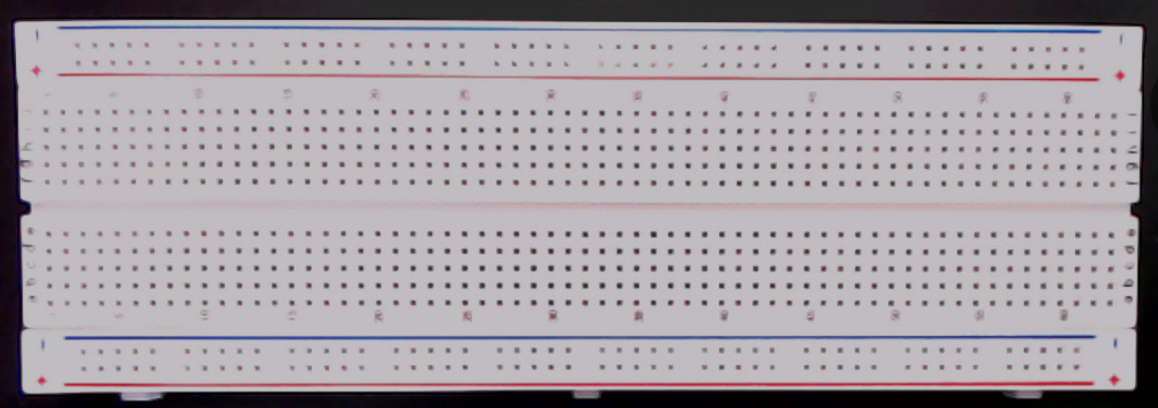
\includegraphics[height=2cm]{breadboard}
    \item One (1) \nano\ (or clone) microcontroller board \\
        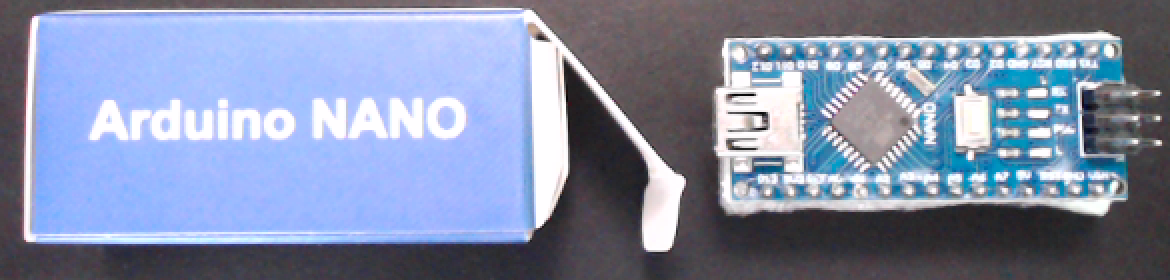
\includegraphics[height=2cm]{nano}
    \item One (1) Mini-USB cable \\
        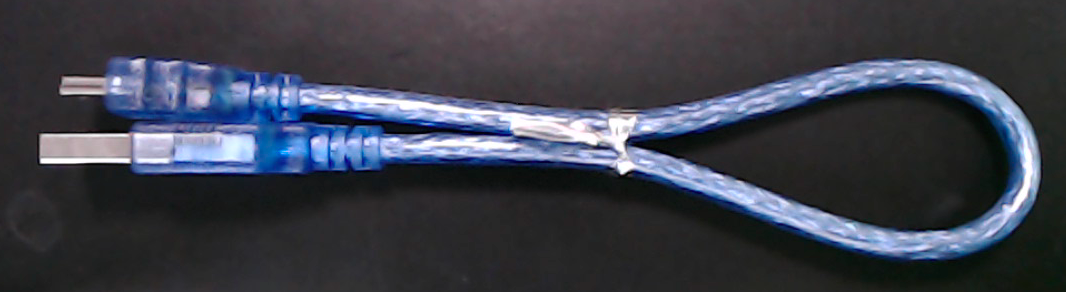
\includegraphics[height=2cm]{usb}
    \item One (1) 74LS20 dual 4-input NAND integrated circuit \\
        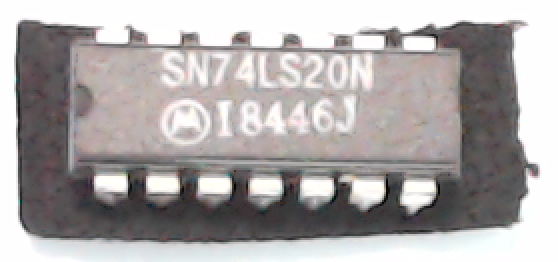
\includegraphics[height=2cm]{nand}
    \item One (1) $4 \times 4$ matrix keypad \\
        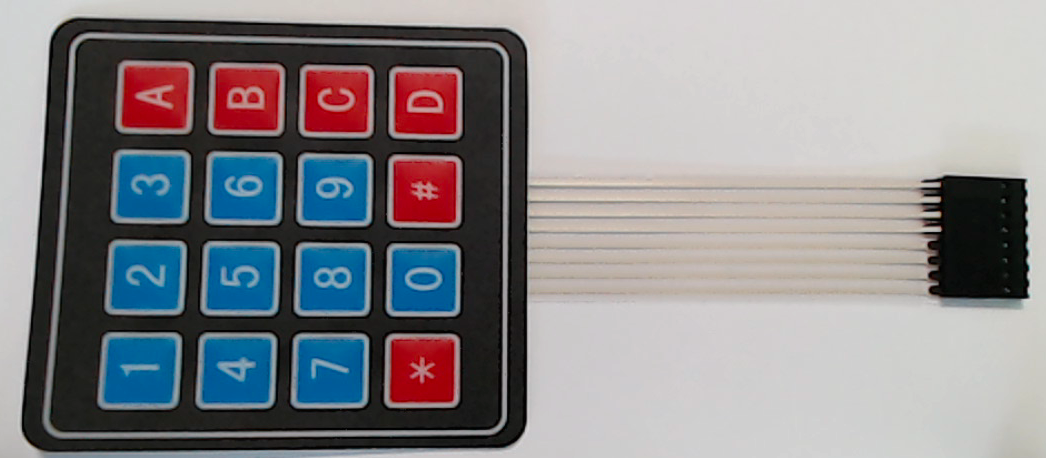
\includegraphics[height=2cm]{keypad}
    \item One (1) 8-pin male-male header strip (might already be inserted into
        keypad's female connectors; might have more than 8 pins) \\
        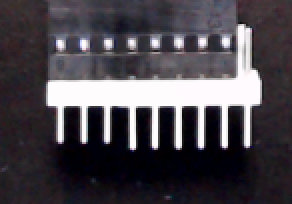
\includegraphics[height=2cm]{header-in-connector} \hspace{1cm} or
        \hspace{1cm} 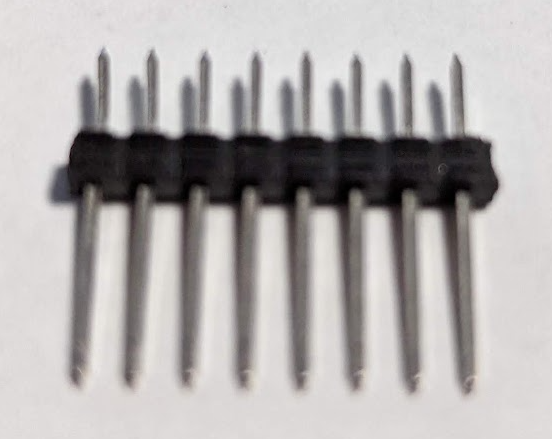
\includegraphics[height=2cm]{header-without-connector}
    \item Two (2) breadboard-mount momentary pushbuttons (might not be attached
        to cardboard strip) \\
        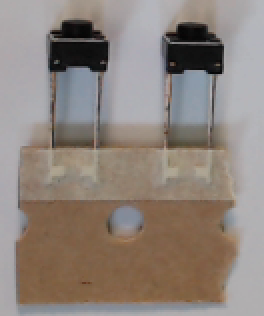
\includegraphics[height=2cm]{buttons}
    \item Two (2) breadboard-mount switches \\
        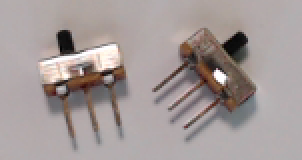
\includegraphics[height=2cm]{sliders}
%    \item One (1) ``MAX7219 8-Digit LED Display 7 Segment Digital Tube'' module
    \item One (1) 8-digit 7-segment display module \\
        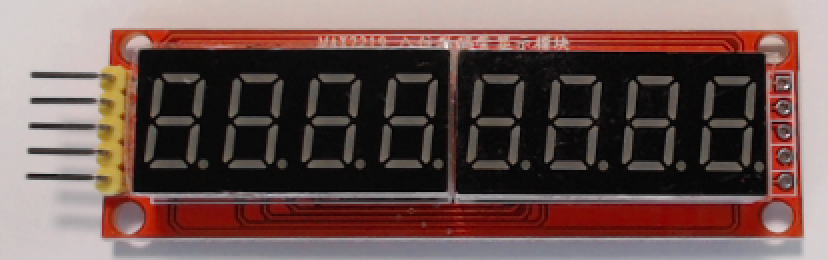
\includegraphics[height=2cm]{display}
    \item One (1) Light Emitting Diode (LED) (color may be different than
        shown) \\
        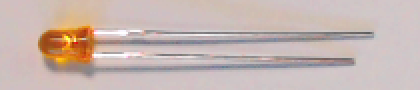
\includegraphics[height=1cm]{led}
    \item One (1) 1k$\Omega$ resistor \\
        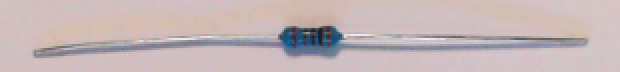
\includegraphics[height=1cm]{resistor}
    \item One (1) 40-conductor 10cm ``rainbow'' cable (male-to-male) \\
        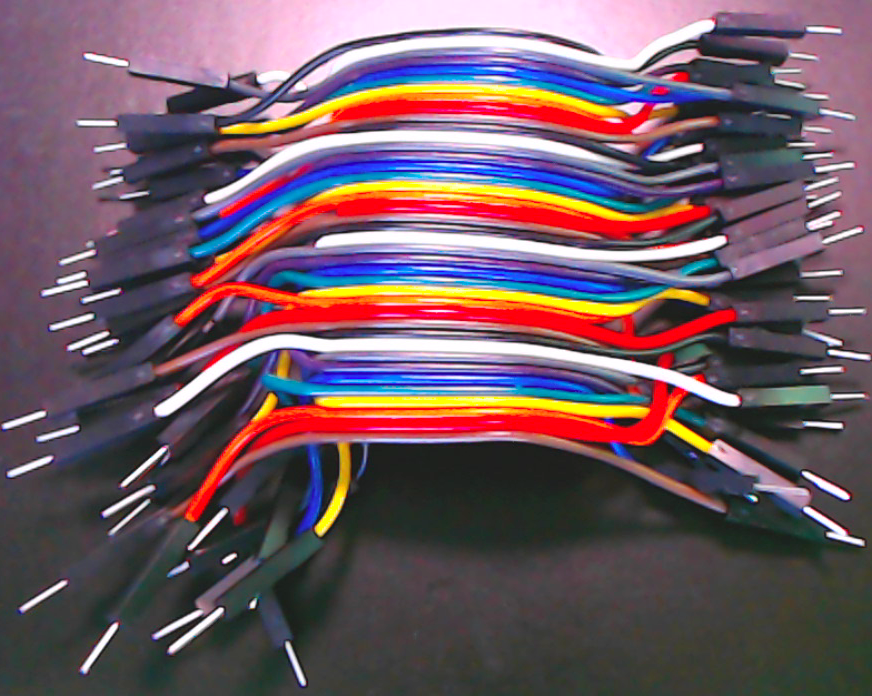
\includegraphics[height=2cm]{mm-cable}
    \item One (1) 5-conductor 20cm ``rainbow'' cable (female-to-male) \\
        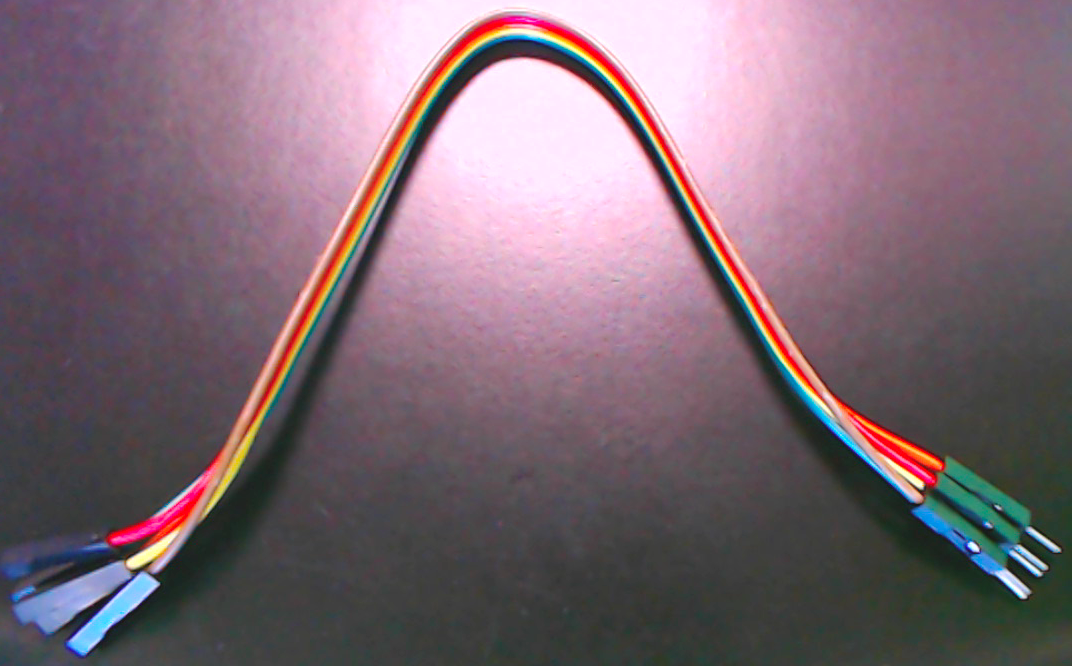
\includegraphics[height=2cm]{fm-cable}
\end{itemize}

\vspace{0.5cm}

\section*{Assembling the Class Kit}

You will assemble the hardware in the following steps. \textbf{At various
checkpoints, you should pause to have a TA or classmate double-check your
work.} When you do so, update the \textit{checkpoints.txt} file to indicate who
checked your work and when they did so.

You may want to store your partially- and fully-completed kit in a plastic food
container or some other container to prevent jumper wires from being pulled out
while in your backpack.

\textit{\textbf{Note:} The following pages include both diagrams and
photographs of the assembly. The wire colors in the diagrams do not match the
wire colors in the assembly. The wire colors in the diagrams are coded by the
purpose they serve, whereas the wire colors in the photographs are the colors
of wires removed from the 40-conductor male-to-male rainbow cable.}

\section{Microcontroller}

A microcontroller, such as the Atmel ATmega328P\footnote{\url{http://ww1.microchip.com/downloads/en/DeviceDoc/Atmel-7810-Automotive-Microcontrollers-ATmega328P_Datasheet.pdf}}
on the \nano, is a very simple processor when compared to a
microprocessor designed for general-purpose computing. At the same time, a
microcontroller has some features not present on a microprocessor, such as
built-in analog-to-digital converters (ADCs).\footnote{We will not use the ADCs
in the I/O labs.} A microcontroller board, such as the \nano, combines
the microcontroller with other components\footnote{Typically, a voltage
regulator, a crystal oscillator, and a USB interface.} in a form factor
convenient for experimentation.

The \nano\ has a mini-USB port to connect to a computer and/or to provide power
to the \nano. The six upward-pointing pins are used to program the \nano\
without using a host computer; we will not use these. It has thirty downward-
pointing pins. \texttt{RX0} and \texttt{TX1} are used for asynchronous serial
communication; as the USB interface also uses the same corresponding pins on
the ATmega328P, we will not use these two pins (you will notice that when the
\nano\ communicates with the host computer, the \texttt{RX} and \texttt{TX}
LEDs will illuminate). Pins \texttt{D2}-\texttt{D13} are digital input/output
pins. Pins \texttt{A0}-\texttt{A7} are analog input pins; however,
\texttt{A0}-\texttt{A5} can also be used as digital input/output pins.
\texttt{AREF} (analog reference) is used to provide a reference voltage for the
ADC (we will not use this pin). Pins \texttt{3V3} and \texttt{5V} provide
regulated 3.3-volt and 5-volt for external circuitry; \texttt{5V} can also be
used to power the \nano\ if connected to a regulated 5V power supply.
\texttt{VIN} can be used to power the \nano\ if connected to an unregulated
power supply, such as a 9V battery; the \nano's onboard voltage regulator will
then provide regulated voltages needed. The \texttt{GND} pins are for the
common ground; the ground portions of external circuitry and of external power
supplies must be electrically connected to the \nano's ground. Finally, the
\texttt{RESET} pins will reset the \nano\ if grounded (pressing the button in
the middle of the \nano\ will also reset the it). Note that, unlike a general-
purpose computer, when a microcontroller is reset it will restart its program
when the reset is released.

The ATmega328P microcontroller on the \nano\ is an 8-bit processor with
32KB of flash memory for the program and 2KB of RAM for data. While 8-bit
logical operations, as well as 8-bit addition and subtraction, can be completed
in one clock cycle, multiplication requires two clock cycles. There is no
hardware divider, and there is no floating point hardware, so integer division
(to include the modulo operation) and all floating point operations are
performed in software, requiring hundreds of clock cycles.

If you have already read the first half of Chapter 8, the ATmega328P has
separate instruction and data memory, similar to the simple processor design
described in the first half of Chapter 8. If you have already read the second
half of Chapter 8, the ATmega328P has a 2-stage pipeline (with \textit{Fetch}
and \textit{Execute} stages). If you have already read Chapter 10, the
ATmega328P does not have cache memory; however, the data memory is SRAM, the
same memory technology used in microprocessors' memory caches. If you have
already read Chapter 10, the ATmega328P does not have a memory management unit
for virtual memory; instead, the ATmega328P uses only physical addressing.

\subsection{Breadboard Terminology}

If you are not familiar with solderless breadboards, read the
\href{https://learn.adafruit.com/breadboards-for-beginners?view=all}{Breadboards for Beginners}
Guide at adafruit.com.

Even though breadboards are often viewed in ``landscape'' orientation (such
as in the photo in Section~\ref{inventory} and as seen in the diagram figures)
instead of ``portrait'' orientation, the numbered sections are called rows and
the lettered sections are called columns. In the interest of preserving common
usage, we will use this terminology. We will refer to specific contact points
using the letter-number combination.

\subsection{Install the Arduino Nano onto the Breadboard}

Orient the breadboard in front of you so that row 1 is on your left and row 63
is on your right; column a should be at the bottom, and column j should be at
the top.

Remove the anti-static foam from the \nano's pins. You will place the
\nano\ on the left side of the breadboard with the USB connector on the
left (that is, facing away from the breadboard). Position the upper row of pins
on contact points g1-g15 and the lower row of pins on contact points c1-c15.
The left side of the \nano\ will obscure the labels for columns c-g. The
right side of the \nano\ will cover contact points c16-g16 but won't use
them. Double-check that:
 \begin{itemize}
    \item the pin labeled \texttt{D12} is in the upper-left, on contact point g1
    \item the pin labeled \texttt{D13} is in the lower-left, on contact point c1
    \item the pin labeled \texttt{VIN} is in the lower-right, on contact point
        c15
    \item the pin labeled \texttt{TX1} is in the upper-right, on contact point
        g15
\end{itemize}

Gently press on both ends of the \nano\ to insert the pins into the
contact points, using a slight rocking motion if necessary
(Figure~\ref{fig:inserting-nano}). Press the \nano\ into the breadboard until it
physically cannot be inserted any deeper (Figure~\ref{fig:nano-inserted}).

\begin{figure}
    \centering
    \subfloat[Press gently on both ends of the \nano.] {
        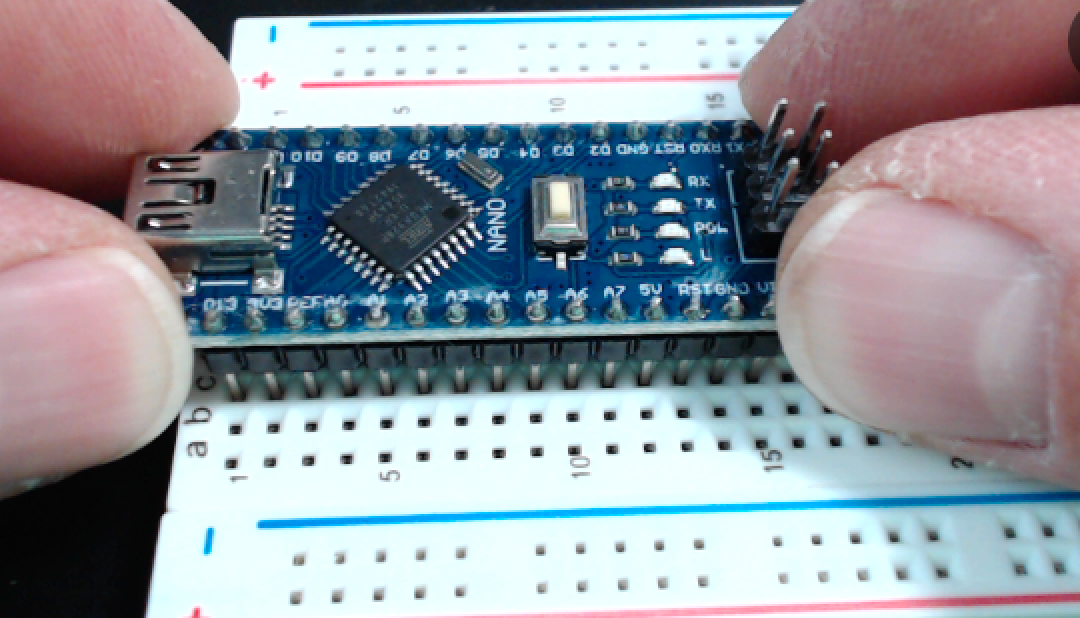
\includegraphics[height=3cm]{inserting-nano}
        \label{fig:inserting-nano}
    }
    \hfil
    \subfloat[The \nano\ fully inserted.] {
        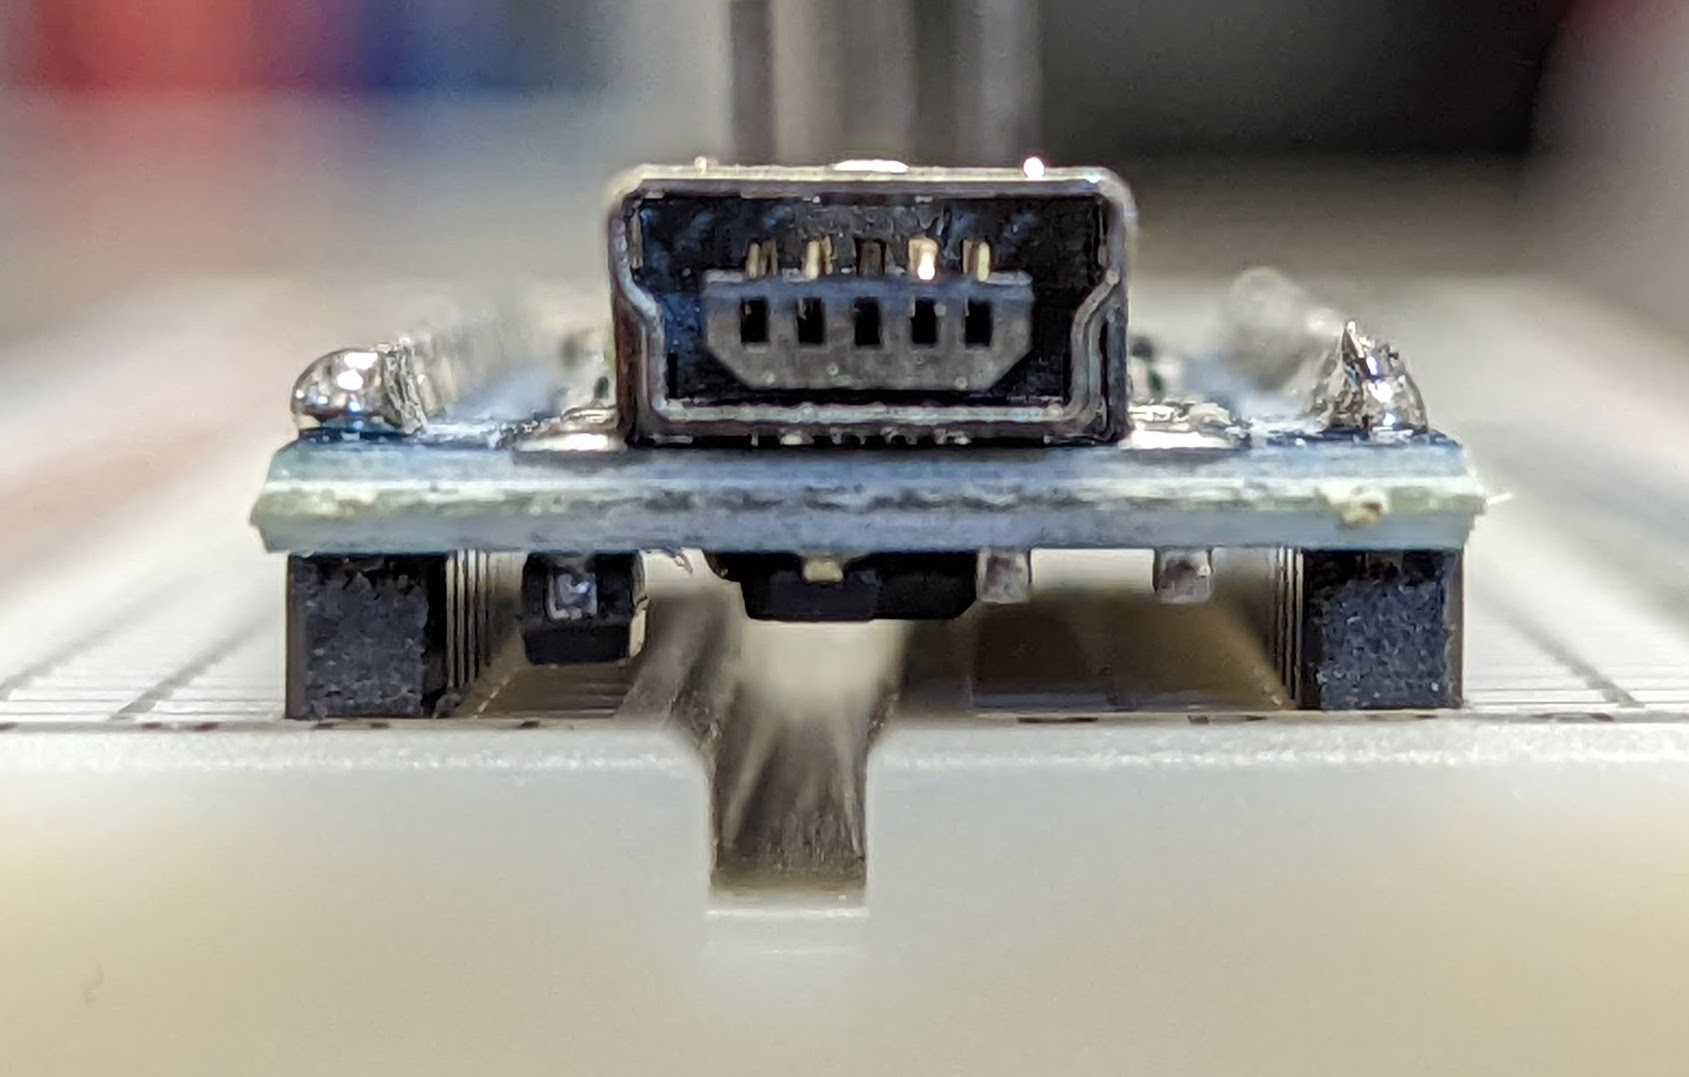
\includegraphics[height=3cm]{nano-fully-inserted}
        \label{fig:nano-inserted}
    }
    \caption{Inserting the \nano\ into the breadboard.}
\end{figure}

\checkpoint{inserted the \nano\ into the breadboard}

\subsection{Optional: Install Arduino IDE}

The Arduino IDE is installed on the lab computers in 015 Avery, 021 Avery, and
the Student Resource Center. If you choose to install the Arduino IDE on your
personal laptop, you can download it from
\url{https://www.arduino.cc/en/software}. Alternatively, you can install a
browser plugin to use the
\href{https://create.arduino.cc/projecthub/Arduino_Genuino/getting-started-with-arduino-web-editor-on-various-platforms-4b3e4a}{Arduino
Web Editor}. There are third-party plugins for many other IDEs; however, using
these may limit our ability to help you if your have difficulties.

\subsubsection*{About Arduino Programs}

An Arduino program is called a \textit{sketch} for historical
reasons.\footnote{The Arduino language is based off of the Wiring language,
which in turn is based off of the Processing language, which was designed to
make computing accessible to artists.} For all intents and purposes, you can
think of it as a C++ program\footnote{Except for the Serial class that we'll
use for debugging purposes, your code in the I/O labs will be C code.} in which
you write two functions, \function{setup} and \function{loop}, along with
any helper code that you need. The file extension for sketches is
\textbf{\textit{.ino}} (as in, Ardu\textbf{\textit{ino}}). The Arduino IDE will
compile your sketch and link it to a \function{main} function that looks
something like:
\begin{lstlisting}
int main() {
    setup();
    while(1) {
        loop();
    }
}
\end{lstlisting}
(The actual \function{main} function\footnote{\url{https://github.com/arduino/ArduinoCore-avr/blob/master/cores/arduino/main.cpp}}
also calls a few other functions from the Arduino core library.)

\subsection{Connect to the \nano}

Connect the USB-B end of the mini-USB cable to a lab computer or to your
personal laptop.\footnote{You can connect it to a ``wall wart'' USB power
supply to run the \nano, but you need to connect it to a computer to upload a
new sketch to the \nano.} Connect the mini-USB end of the cable to your \nano.
The \texttt{PWR} LED will light up, and you may see the \texttt{L} LED
repeatedly blink on-and-off. The \texttt{L} LED is connected to the \nano's pin
D13, and Arduino microcontroller boards typically leave the factory with
\textit{Blink.ino} loaded, but these \nano{}s do not appear to have
\textit{Blink.ino} pre-loaded (this is inconsequential).

\begin{lstlisting}[basicstyle=\ttfamily\footnotesize]
// the setup function runs once when you press reset or power the board
void setup() {
  // initialize digital pin LED_BUILTIN as an output.
  pinMode(LED_BUILTIN, OUTPUT);
}

// the loop function runs over and over again forever
void loop() {
  digitalWrite(LED_BUILTIN, HIGH);   // turn the LED on (HIGH is the voltage level)
  delay(1000);                       // wait for a second
  digitalWrite(LED_BUILTIN, LOW);    // turn the LED off by making the voltage LOW
  delay(1000);                       // wait for a second
}
\end{lstlisting}

Open the Arduino IDE on the computer that your \nano\ is connected to. Connect
the Arduino IDE to the \nano. If you are using Arduino IDE 1.8, see this
\href{https://www.arduino.cc/en/Guide/ArduinoNano#select-your-board-type-and-port}{Tutorial}
for selecting the \nano\ board, processor, and COM port (or this
\href{https://www.arduino.cc/en/Guide/ArduinoUno#select-your-board-type-and-port}{Tutorial
for the Arduino Uno}, which has more detail on selecting the COM port). If you
are using Arduino IDE 2.0 or the Arduino Web Editor, COM port should be
automatically detected; however, you will still need to select the board and
processor; see Figure~\ref{fig:selecting-nano} and the discussion in
Section~\ref{sec:processor-selection}.

\begin{figure}
    \centering
    \subfloat[Selecting the board with Arduino IDE 1.8.] {
        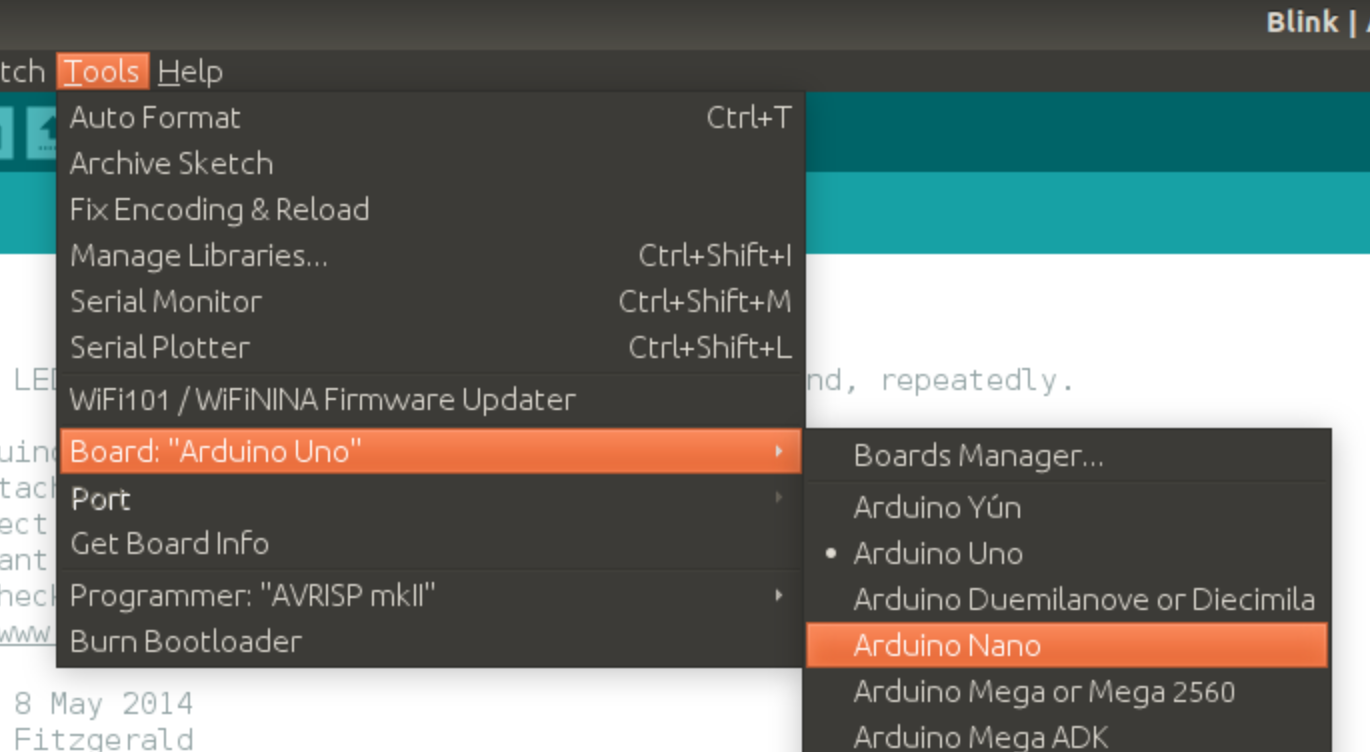
\includegraphics[width=7cm]{selecting-board-1_8_5}
        \label{fig:selecting-board-1}
    }
    \hfil
    \subfloat[Selecting the board with Arduino IDE 2.0.] {
        % 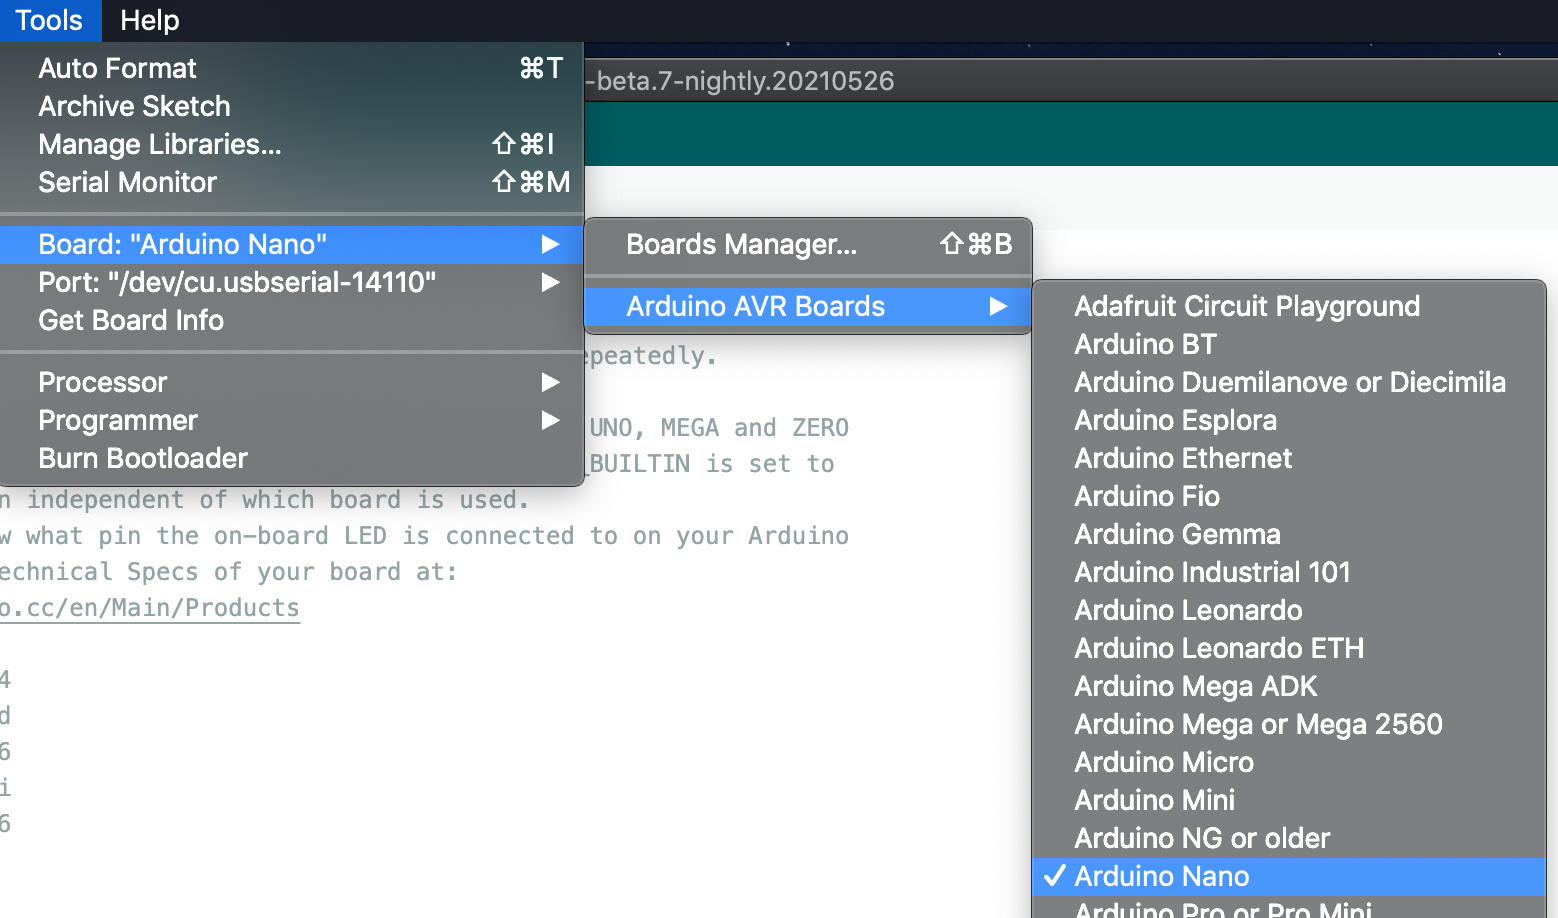
\includegraphics[width=7cm]{selecting-board-from-menu}
        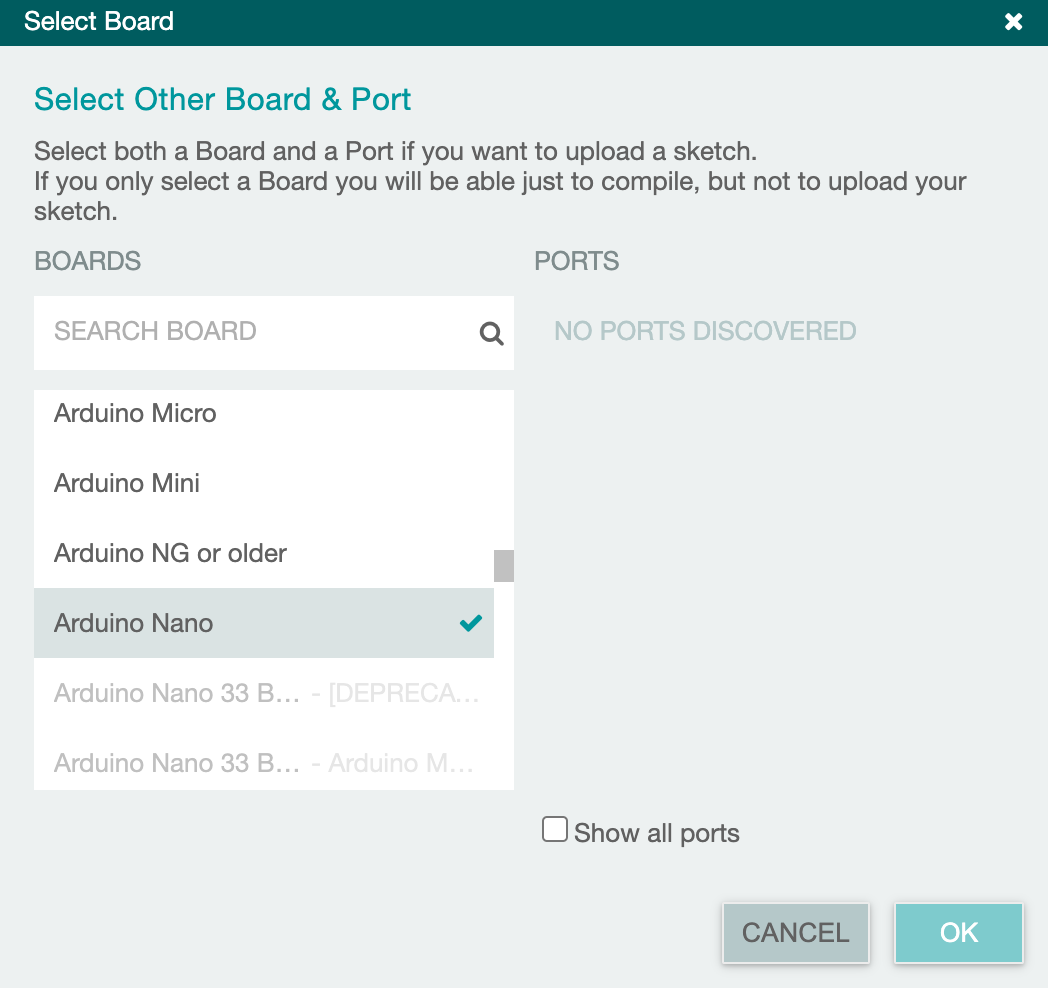
\includegraphics[height=4.1cm]{selecting-board}
        \label{fig:selecting-board-2}
    }

    \subfloat[Selecting the processor after selecting the board.] {
        % \vtop{\vskip-4.1cm\hbox{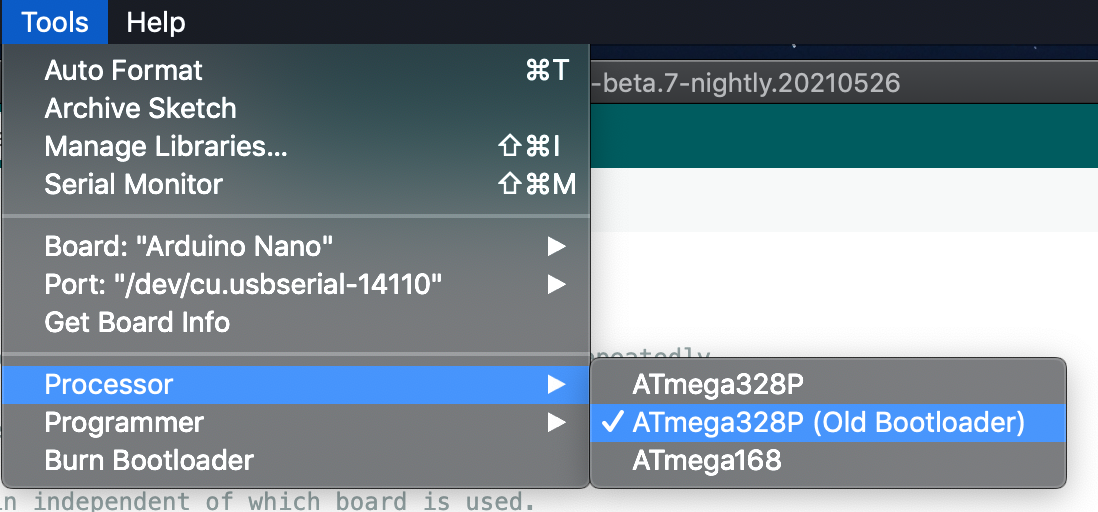
\includegraphics[width=5cm]{selecting-processor}}}
        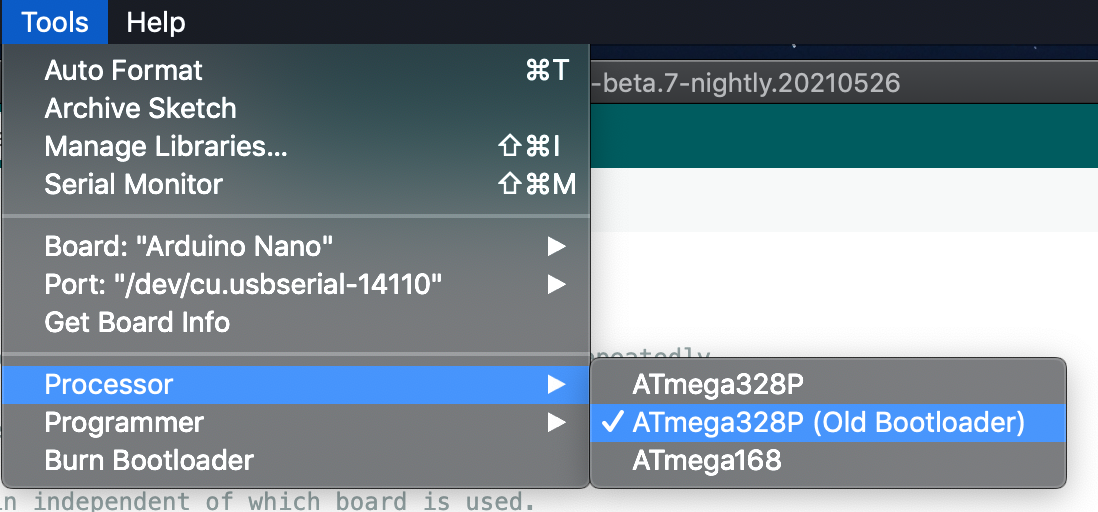
\includegraphics[width=7cm]{selecting-processor}
        \label{fig:selecting-processor}
    }
    \caption{Selecting board and processor in the Arduino IDE.
        \label{fig:selecting-nano}}
\end{figure}

\subsubsection{Selecting the Correct ``Processor''}\label{sec:processor-selection}

There are \textit{three} choices for the \nano{}'s processor, two of which
specify the ATmega328P processor. Even though the difference is a USB
interface issue, it is resolved through the Arduino IDE's ``Processor''
selection:

\begin{itemize}
\item Official \nano{}s manufactured in 2018 and later use the FT232RL USB
    interface chip. Under the ``Tools'' menu, when choosing ``Processor'',
    select ``ATmega328P''.
\item \nano{}s manufactured in 2017 and earlier, and \textit{many} \nano\
    clones, use the CH340 USB interface chip. Under the ``Tools'' menu, when
    choosing ``Processor'', select ``ATmega328P (Old Bootloader)''. (If you are
    using the Arduino IDE 1.8.4 and earlier, which don't have the ``(Old
    Bootloader)'' option, simply select ``ATmega328P'').
\item If your \nano\ has the ATmega168 processor, replace it with one that has
    an ATmega328P processor. While the processor differences shouldn't be
    problem in the I/O labs, the older \nano{}s that use the ATmega168 have a
    slightly different pin-out that will affect constructing your class kit.
\end{itemize}

\subsubsection{Updating USB Driver if Necessary}

We have seen some Windows computers without the CH340 USB driver. If you
encounter this problem and the Device Manager shows you the warning in
Figure~\ref{fig:usb-warning}, then the first thing to try is updating the
driver. Right-click on USB2.0-Seri! (Figure~\ref{fig:update-driver}) and choose
``Update driver''. Then choose ``Search automatically for updated driver
software''.

\begin{figure}
    \centering
    \subfloat[] {
        
\includegraphics[width=.4\textwidth]{usb-drivers/device-manager-warning}
        \label{fig:usb-warning}
    }
    \hfil
    \subfloat[] {
        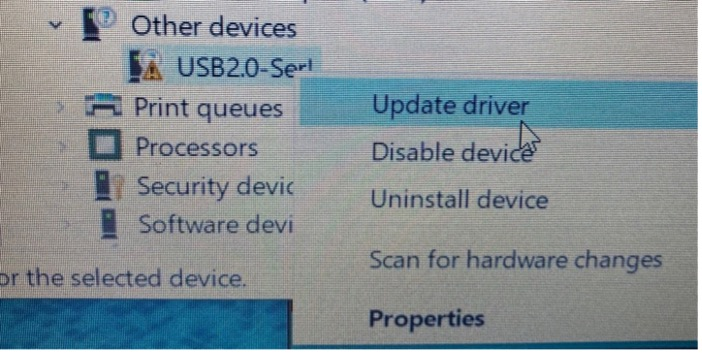
\includegraphics[width=.4\textwidth]{usb-drivers/update-driver}
        \label{fig:update-driver}
    }

    \caption{Selecting board and processor in the Arduino IDE.}
\end{figure}

If Windows reports that ``Windows has successfully updated your drivers'' then
you should now be able to connect to the \nano. On the other hand, if Windows
reports that ``Windows was unable to install your USB2.0-Ser!'', then the
\href{https://learn.sparkfun.com/tutorials/how-to-install-ch340-drivers/}{How
to Install CH340 Drivers} page at sparkfun.com will guide you through manually
downloading the driver and installing it.

Sparkfun's \href{https://learn.sparkfun.com/tutorials/how-to-install-ch340-drivers/}
{How to Install CH340 Drivers} page also has instructions for installing the
driver on MacOS and on Linux; however, we are not aware of any students needing
to manually install the CH340 driver on MacOS.

\subsubsection{No Driver Warning but Cannot Connect}

Probably what happened is that your computer has the driver but you're telling
the IDE to connect to the wrong virtual COM port. Tye typical way to handle this
is to disconnect the \nano\ from your computer, go to the part of the menu where
you connect to the COM port, connect the \nano\ to your computer, and select
whichever COM port appears after plugging in the \nano.

\subsection{Upload a New Sketch}

From the Arduino IDE's menu, open the \textit{Blink.ino} example: \\
\textit{File} $\rightarrow$ \textit{Examples} $\rightarrow$ \textit{01.Basics} $\rightarrow$ \textit{Blink} \\
Select \textit{Save As...} and save the project as \textit{MyBlink}.

Edit the values in the \function{delay} calls to change the delays between the
LED turning on, off, and on again. Select values that will visibly have a
difference, such as 250 or 2000. Compile the program using the ``Verify''
checkmark in the IDE's toolbar and make corrections if the program doesn't
compile. Upload the program to your \nano\ using the ``Upload'' arrow in the
IDE's toolbar. (If you forget to compile first, the IDE will compile your
program before uploading, but I find it useful to find compile-time mistakes
before attempting to upload the program.)

If you successfully uploaded \textit{MyBlink.ino} then you will see the
following in the IDE's \textit{Output} window:
\begin{quote}
\dots (elided configuration data)\dots
\begin{verbatim}
avrdude: AVR device initialized and ready to accept instructions

Reading | ################################################## | 100% 0.01s

avrdude: Device signature = 0x1e950f (probably m328p)
avrdude: reading input file "/var/folders/p7/lx4gt70d0_34cpy8r0j3c95c0000gp/T/arduino-sketch-11A4823C54657006C9F78B0812B621A8/MyBlink.ino.hex"
avrdude: writing flash (932 bytes):

Writing | ################################################## | 100% 0.33s

avrdude: 932 bytes of flash written

avrdude done.  Thank you.


--------------------------
upload complete.
\end{verbatim}\end{quote}
and then the LED's on-off pattern will change, reflecting the \function{delay}
values you assigned (Figure~\ref{fig:myblink}).

\subsubsection*{Handling Errors}

If you get an error when attempting to upload a sketch, try these corrective
measures:

\begin{enumerate}
    \item Double-check that you have ``ATmega328P (Old Bootloader)'' selected
        (see Figure~\ref{fig:selecting-processor}).
    \item Try uploading again (if you attempt to upload a sketch too soon after
        connecting your \nano\ to your computer, the USB interface won't have
        finished its handshake).
    \item The \href{https://support.arduino.cc/hc/en-us/articles/4401874331410--Error-avrdude-when-uploading}{Troubleshooting
        Guide} recommends disconnecting your \nano\ and reconnecting it, then
        selecting whichever COM port appears.
\end{enumerate}

If, instead of an error, your IDE ``hangs'' while collecting configuration data, try this corrective measure:

\begin{itemize}
\item Press the \texttt{RESET} button in the middle of the \nano; the IDE
    should begin uploading the sketch after you release the button.
\end{itemize}

\begin{figure}
    \centering
    \animategraphics[autoplay,loop,height=5cm]{8}{animations/myblink-}{0}{6}
    \caption{\textit{MyBlink.ino} has a different on-off
        pattern than \textit{Blink.ino}.\label{fig:myblink}}
\end{figure}

\checkpoint{uploaded new code to the \nano}

\section{Output Devices}

\subsection{Connect Power and Ground to Power Bus Strips}

The columns marked with red and blue stripes are the power bus strips, also
known as the power rails. You will now provide power to the bus strips so that
the other components can use power.

\disconnect\

Take the 40-conductor \rainbow, and peel off two wires together. In the
interest of keeping track of which wires are used for which purposes, it would
be best to leave the two wires attached to each other as a 2-conductor cable
(Figure~\ref{fig:two-wires}). At one end of this 2-conductor cable, insert one
lead into contact point a12 (notice that contact point a12 is electrically
connected to the \nano's \texttt{5V} pin, which is in contact point c12) and
the other into contact point A14 (notice that contact point A14 is electrically
connected to one of the \nano's \texttt{GND} pins, which is in contact point
c14); see Figure~\ref{fig:power-step-1}. Insert the other end of the
\texttt{5V} wire into the lower \power\ marked with a red stripe. Insert the
other end of the \texttt{GND} wire into the lower \ground\ marked with a blue
stripe; see Figure~\ref{fig:power-step-2}.

\begin{figure}
    \centering
    \subfloat[]{
        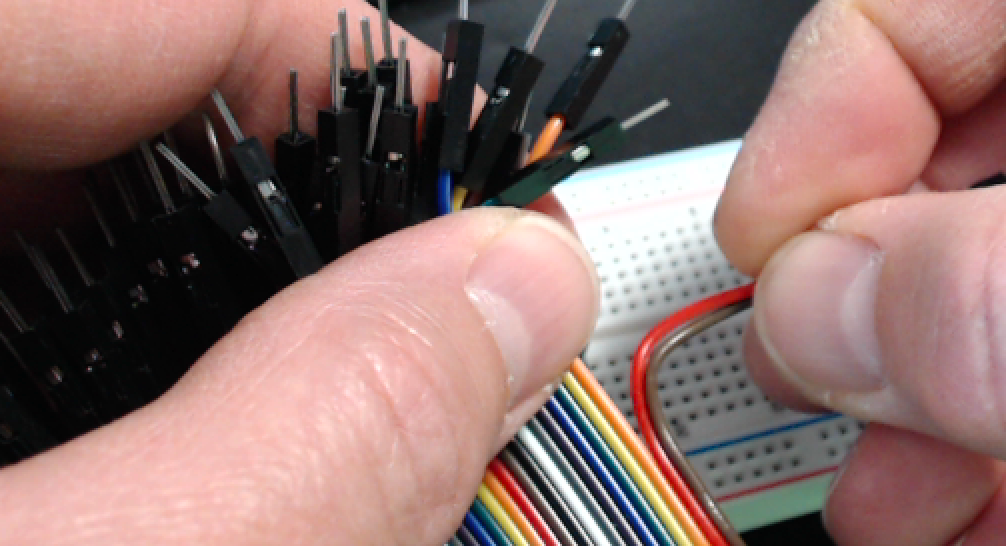
\includegraphics[width=0.4\textwidth]{removing-two-wires}
    }
    \hfil
    \subfloat[]{
        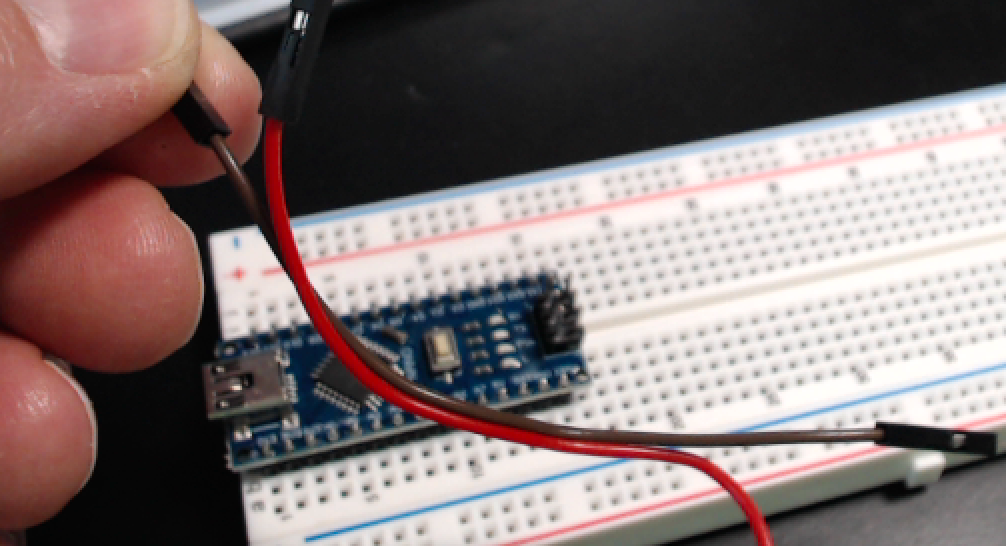
\includegraphics[width=0.4\textwidth]{two-wires}
    }
    \caption{Removing a two-conductor cable from the 40-conductor cable.\label{fig:two-wires}}
\end{figure}

\begin{figure}
    \centering
    \subfloat[Tapping power and ground from the \nano.]{
        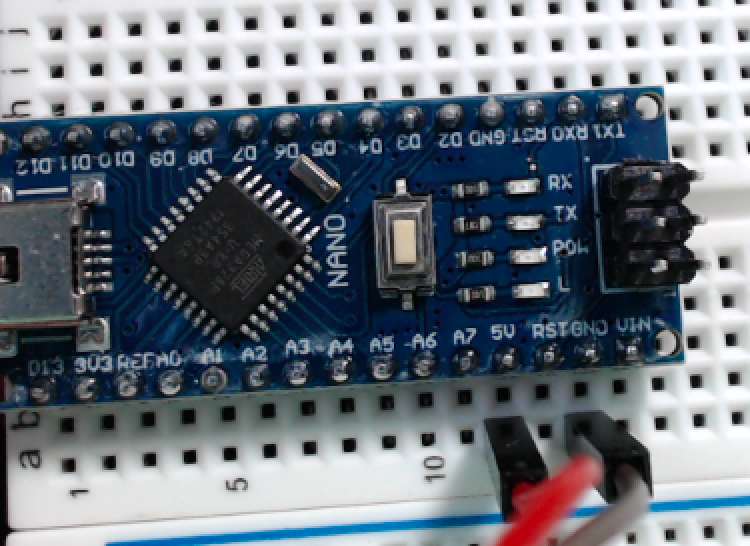
\includegraphics[width=0.27\textwidth]{power-step-1}
        \label{fig:power-step-1}
    }
    \hfil
    \subfloat[Connecting lower power bus to power and ground.]{
        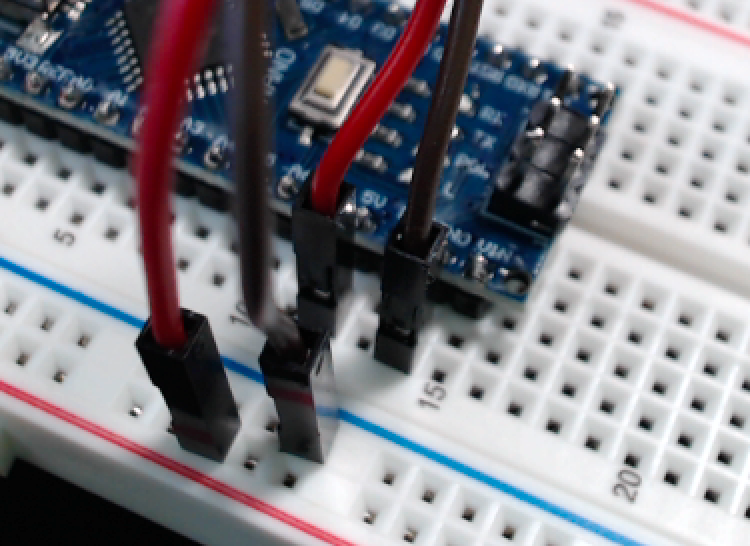
\includegraphics[width=0.27\textwidth]{power-step-2}
        \label{fig:power-step-2}
    }
    \hfil
    \subfloat[Connecting upper and lower power busses.]{
        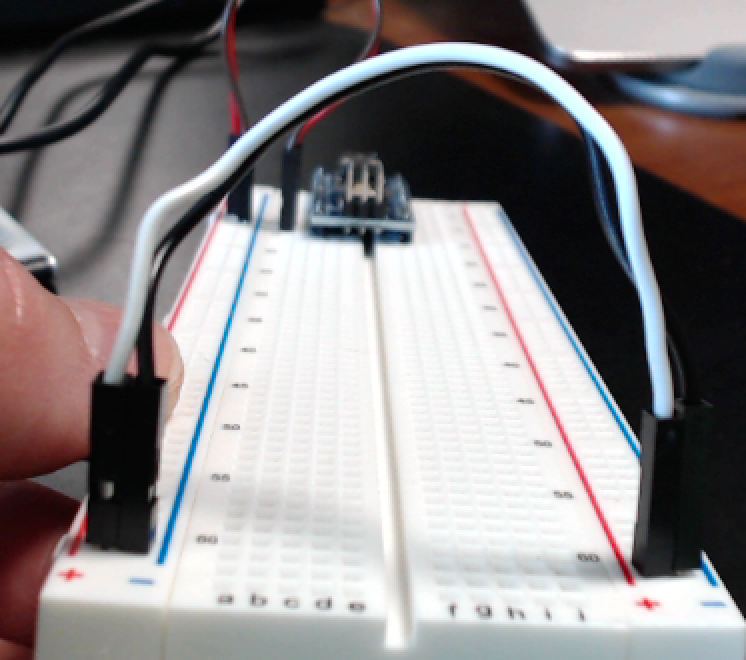
\includegraphics[width=0.27\textwidth]{power-step-3}
        \label{fig:power-step-3}
    }
    \caption{Providing power and ground to power busses.}
\end{figure}

Peel off another 2-wire cable from the \rainbow. Use this 2-conductor cable to
connect the lower \power\ to the upper \power, and to connect the lower
\ground\ to the upper \ground. If you place this cable on the right end of the
breadboard, it will be out of the way during the remaining steps; see
Figure~\ref{fig:power-step-3}.

\checkpoint{connected the \power{}s and the \ground{}s}

\subsection{Light Emitting Diode}

You will now connect an external LED. An LED is a \textit{light emitting diode},
and like all diodes it allows current to flow only in one direction. As shown
in Figure~\ref{fig:led-annotated}, one lead on the LED is longer than the
other, and this tells us which direction current will flow. When we insert the
LED into the circuit, power will flow from one of the \nano's pins through the
LED to ground. Most LEDs have so little internal resistance that, unless
current is otherwise limited, enough current will flow through the LED to
destroy the semiconductor material. The typical solution, which we will use, is
to employ a \textit{current-limiting resistor}. (If you look very closely at
your \nano, you will see a tiny surface-mount resistor next to each built-in
LED.)

Figure~\ref{fig:led-diagram} shows a diagram of of the components you will
install for the LED output.

\begin{figure}
    \centering
    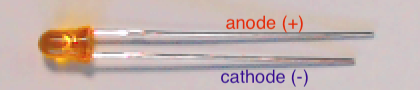
\includegraphics[height=2cm]{led-annotated}
    \caption{The LED's longer lead connects to power; the shorter lead connects
        to ground.\label{fig:led-annotated}}
\end{figure}

\begin{figure}
    \centering
    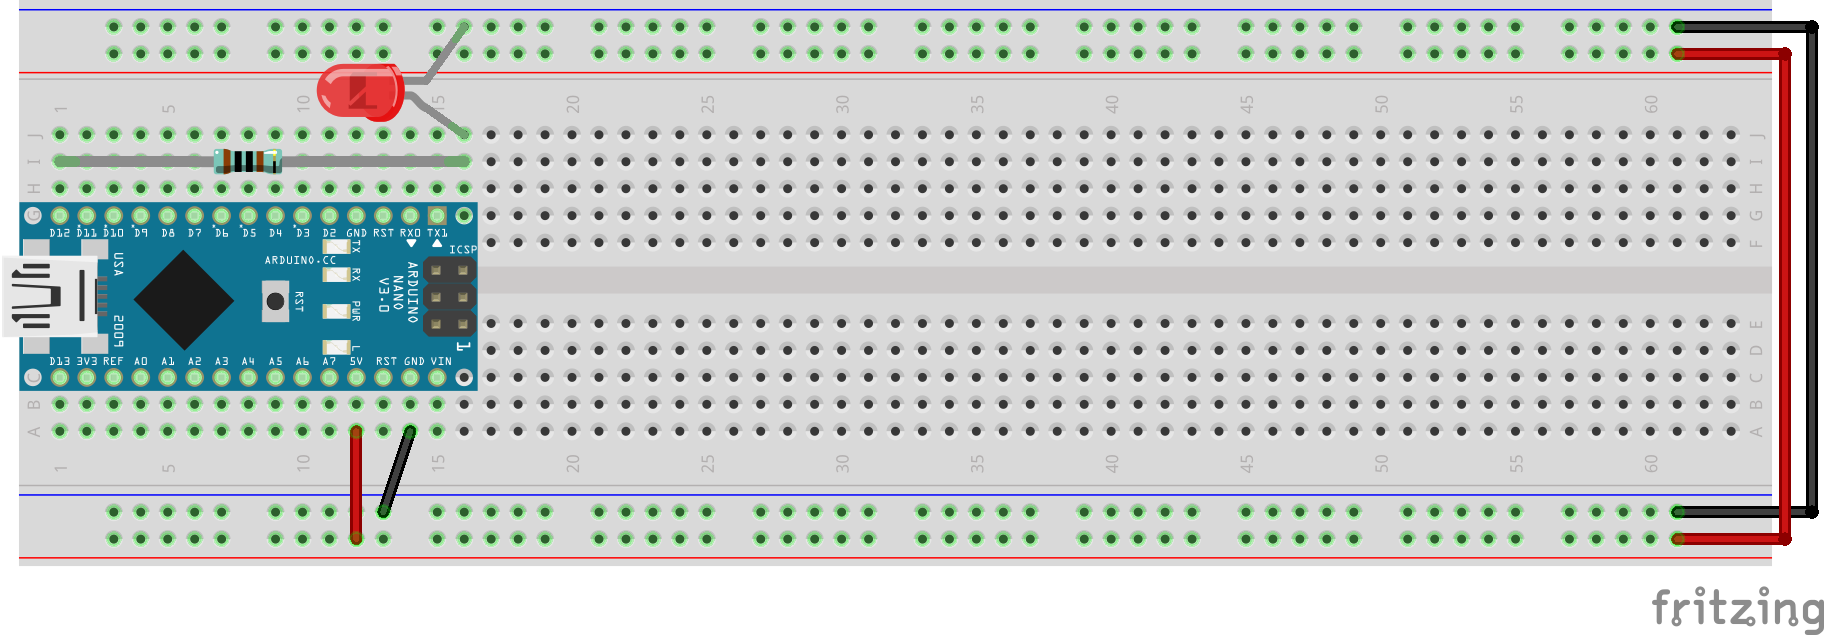
\includegraphics[width=0.9\textwidth]{fritzing_images/led}
    \caption{Diagram of component assembly for LED output.
        \label{fig:led-diagram}}
\end{figure}

Take the 1k$\Omega$ resistor and place a right-angle bend in each lead about
0.4in (1cm) from the ends (we want the remaining length to be about 1.5in
(3.8cm) -- you do not need to be exact;\footnote{If you want to try to be
exact, you can use the breadboard's contact points to measure: they are 0.1in
(2.54mm) apart.} the leads are flexible enough that you only need to be
approximate) -- see Figure~\ref{fig:resistor-bent}. Insert one of the resistor's
leads into contact point i1 (electrically connected to the \nano's \texttt{D12}
pin in g1) and the other into contact point i16. Gently press along the length
of the resistor, causing the leads to deform slightly, until the resistor's
height above the breadboard is about the same as the \nano's printed circuit
board. See Figure~\ref{fig:resistor-inserted}.

Take the LED and spread the leads apart slightly. Insert the longer lead (the
anode) in contact point j16, and the shorter lead (the cathode) in the upper
\ground. See Figure~\ref{fig:led-inserted}.

\begin{figure}
    \centering
    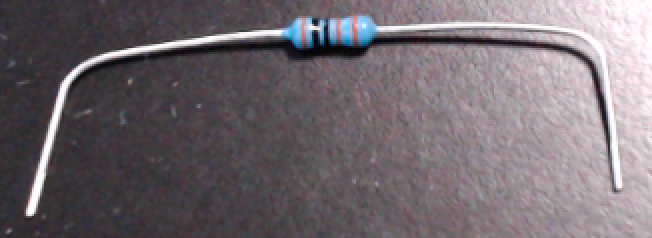
\includegraphics[height=2cm]{resistor-bent}
    \caption{Bend the resistor's leads about 1cm from the ends.\label{fig:resistor-bent}}
\end{figure}

\begin{figure}
    \centering
    \subfloat[The resistor run between contact points i1 and i16.]{
        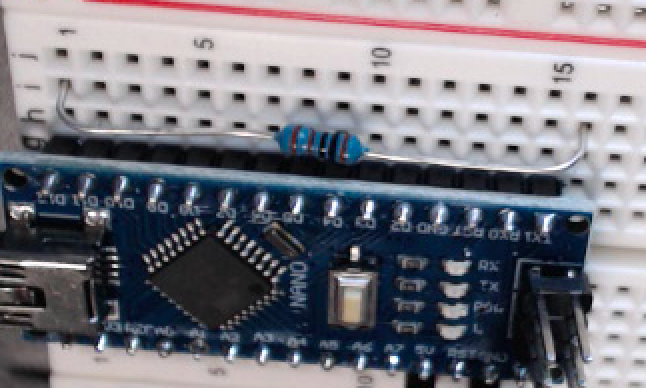
\includegraphics[width=0.65\textwidth]{resistor-inserted}
        \label{fig:resistor-inserted}
    }
    \hfil
    \subfloat[The LED's longer lead is in contact point j16, and its shorter lead is in the \ground.]{
        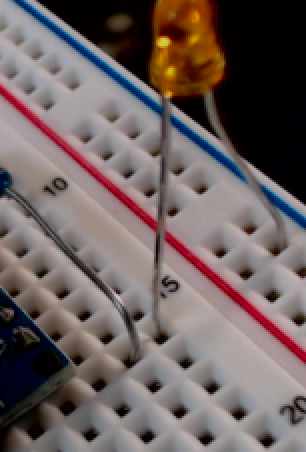
\includegraphics[width=0.25\textwidth]{led-inserted}
        \label{fig:led-inserted}
    }
    \caption{Constructing the LED assembly.}
\end{figure}

When you have finished installing the external LED, there should be the
electrical connections described in Table~\ref{tab:led}.

\begin{table}
    \begin{center}\begin{tabular}{||c|c|c|c||} \hline\hline
    LED lead    & Resistor lead & \nano\ pin    & Pulled High/Low \\ \hline
    Anode       & Right         &               & \\
    Cathode     &               &               & Pulled Low \\
                & Left          & \texttt{D12}  & \\ \hline\hline
    \end{tabular}\end{center}
    \caption{Electrical Connections for External LED.\label{tab:led}}
\end{table}

\checkpoint{installed the LED and its current-limiting resistor}

In the Arduino IDE, load \textit{MyBlink.ino}. In the \function{pinMode} and
the two \function{digitalWrite} calls, replace the \lstinline{LED_BUILTIN}
argument with \lstinline{12}:
\begin{lstlisting}
void setup() {
  pinMode(12, OUTPUT);
}

void loop() {
  digitalWrite(12, HIGH);
  delay(250);   // or whatever value you used
  digitalWrite(12, LOW);
  delay(1500);  // or whatever value you used
}
\end{lstlisting}
Re-connect the USB cable to your \nano. Compile the sketch and upload it to
your \nano. Now, instead of the built-in LED, the external LED that you
installed will blink (Figure~\ref{fig:revisedblink}).

\begin{figure}
    \centering
    \animategraphics[autoplay,loop,height=5cm]{8}{animations/revisedblink-}{0}{6}
    \caption{The revised \textit{MyBlink.ino} causes the external LED to
        blink.\label{fig:revisedblink}}
\end{figure}

\subsection{Seven-Segment Display Module}

Examine the 7-segment display module. Notice that the header has five pins
(Figure~\ref{fig:display-module-header}): \texttt{VCC} (common collector
voltage), \texttt{GND} (ground), \texttt{DIN} (data in), \texttt{CS} (chip
select), and \texttt{CLK} (clock). When the display module is oriented for
viewing, these header pins will be on the left.

Figure~\ref{fig:display-diagram} shows a diagram of of the wiring to connect
the display module to the breadboard.

\begin{figure}
    \centering
    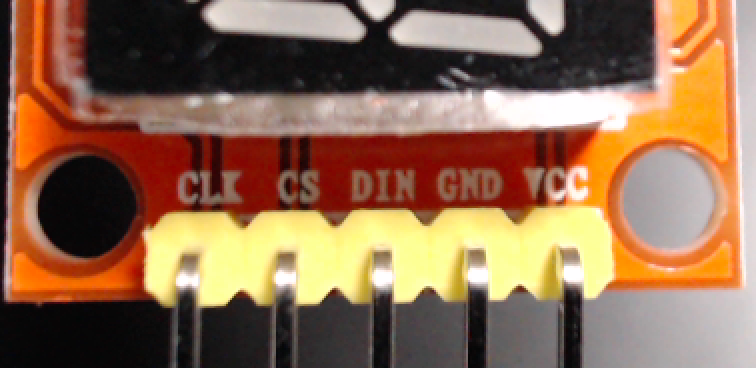
\includegraphics[width=5cm]{display-module-header}
    \caption{The display module's header has five pins.
        \label{fig:display-module-header}}
\end{figure}

\begin{figure}
    \centering
    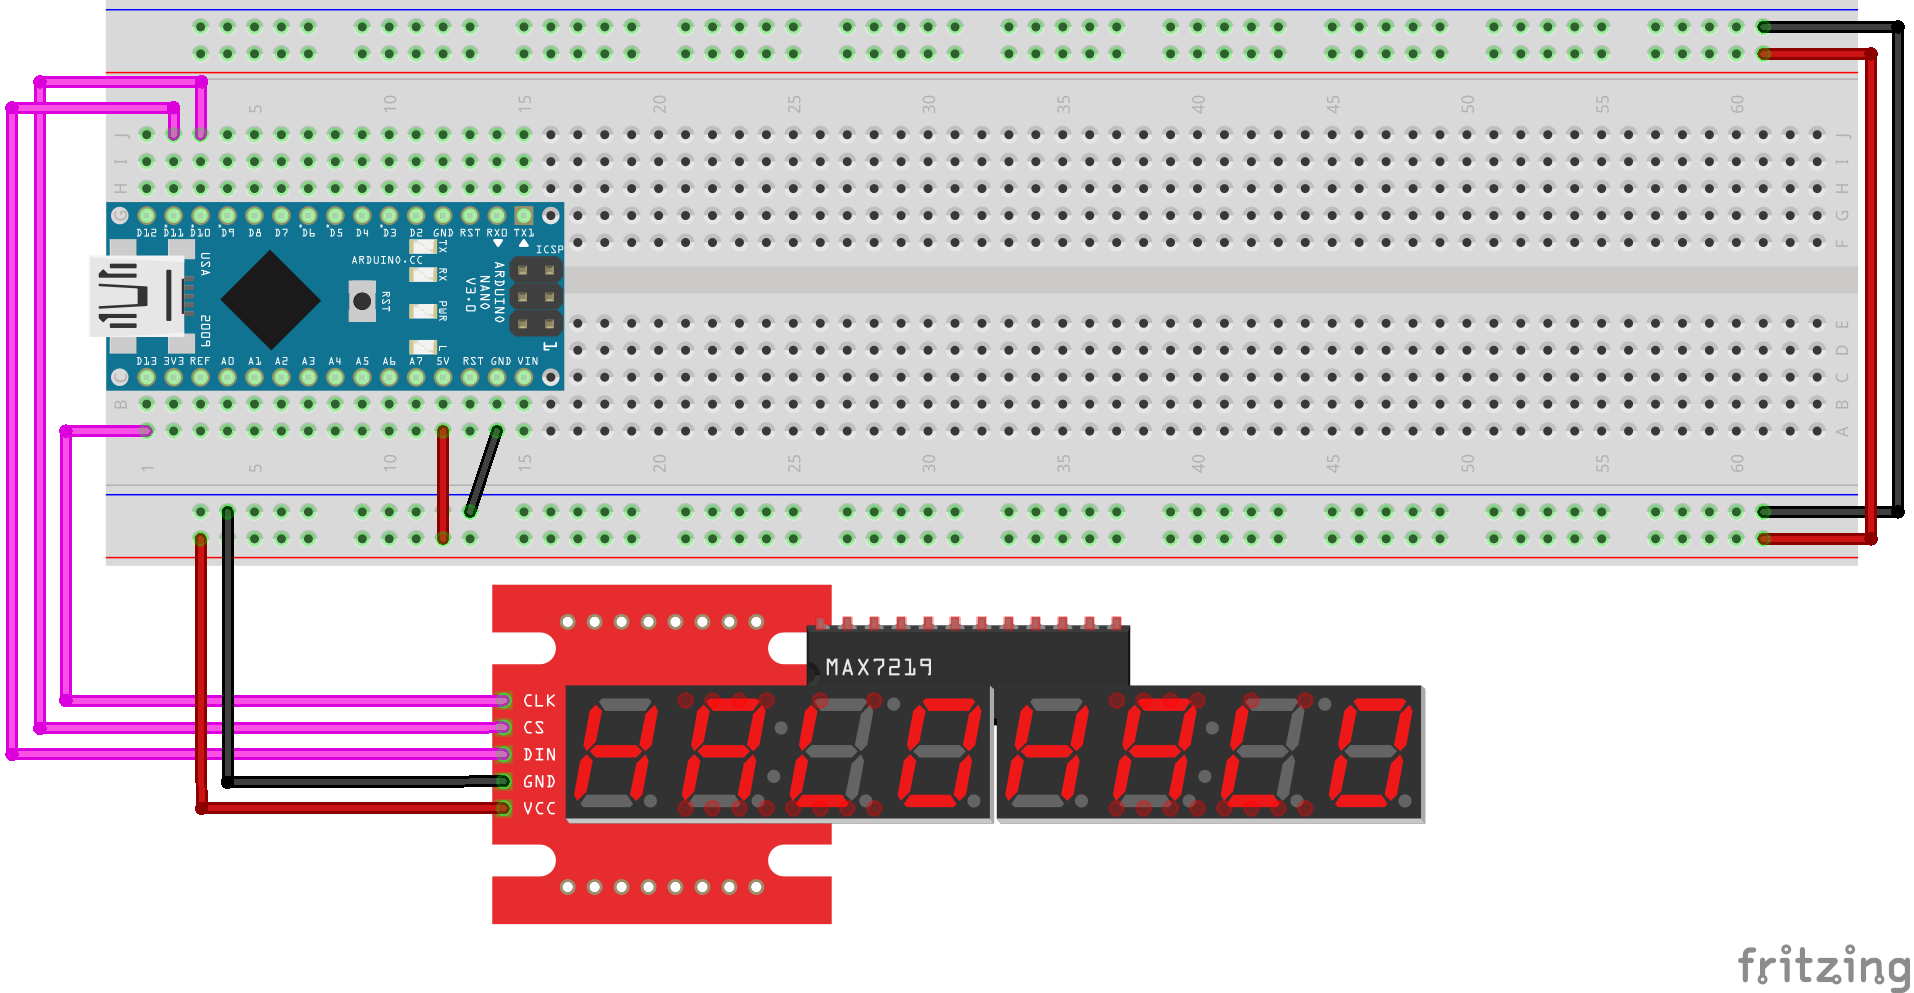
\includegraphics[width=0.9\textwidth]{fritzing_images/display}
    \caption{Diagram of display module's connections to the breadboard.
        \label{fig:display-diagram}}
\end{figure}

\disconnect\

Take the 5-conductor female-to-male rainbow cable and attach the five female
connectors to the display module's five header pins; see
Figure~\ref{fig:display-module-female-connectors}.

As you insert the male connectors into the breadboard, you may have to
partially separate the wires at the male end. In the interest of keeping track
of which wires are used for which purposes, do not fully separate the wires.
Identify the wire that is connected to the display module's \texttt{CLK} pin;
insert the male end of this wire in contact point a1 (electrically connected to
the \nano's \texttt{D13} pin in c1); see Figure~\ref{fig:display-module-CLK}.
Insert the male end of the \texttt{CS} wire into contact point j3 (electrically
connected to the \nano's \texttt{D10} pin in g3); see
Figure~\ref{fig:display-module-CS}. Insert the male end of the \texttt{DIN}
wire into contact point j2 (electrically connected to the \nano's \texttt{D11}
pin in g2); see Figure~\ref{fig:display-module-DIN}. Insert the \texttt{GND}
wire into a \ground, and the \texttt{VCC} wire into a \power\
(Figure~\ref{fig:display-module-power}).

\begin{figure}
    \centering
    \subfloat[Connect the female ends of the 5-conductor cable to the display module's header pins (your colors may be different).] {
        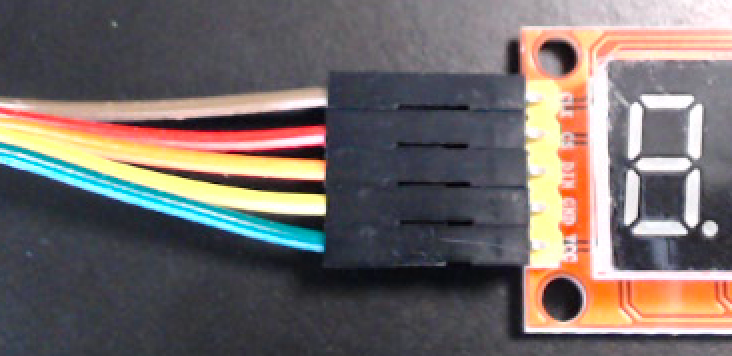
\includegraphics[width=0.27\textwidth]{display-module-female-connectors}
        \label{fig:display-module-female-connectors}
    }
    \hfil
    \subfloat[The display module's clock will be driven by \texttt{D13}.] {
        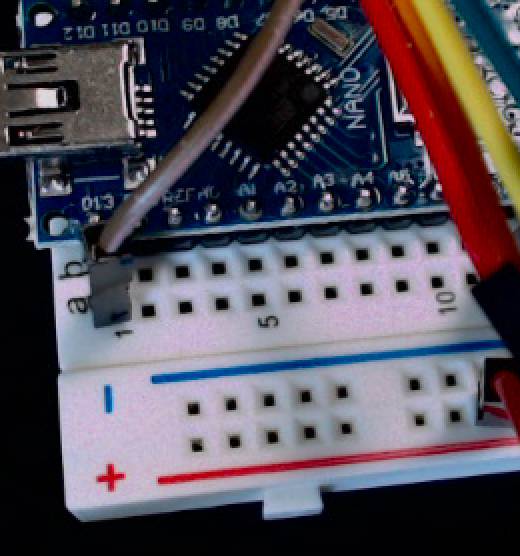
\includegraphics[width=0.27\textwidth]{display-module-CLK}
        \label{fig:display-module-CLK}
    }
    \hfil
    \subfloat[The display module's chip-select will be driven by
        \texttt{D10}.] {
        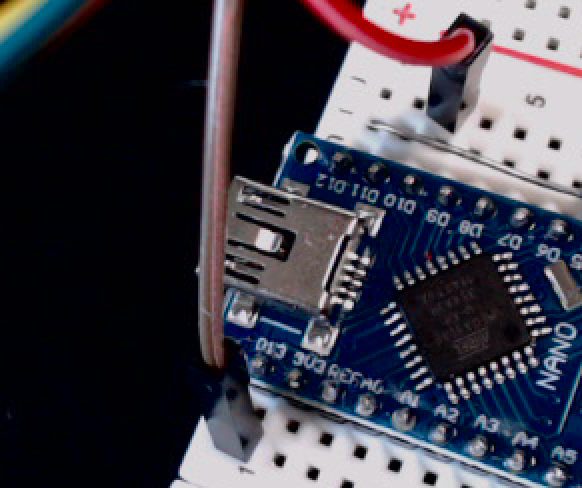
\includegraphics[width=0.27\textwidth]{display-module-CS}
        \label{fig:display-module-CS}
    }

    \subfloat[The display module's data-in will be driven by \texttt{D11}] {
        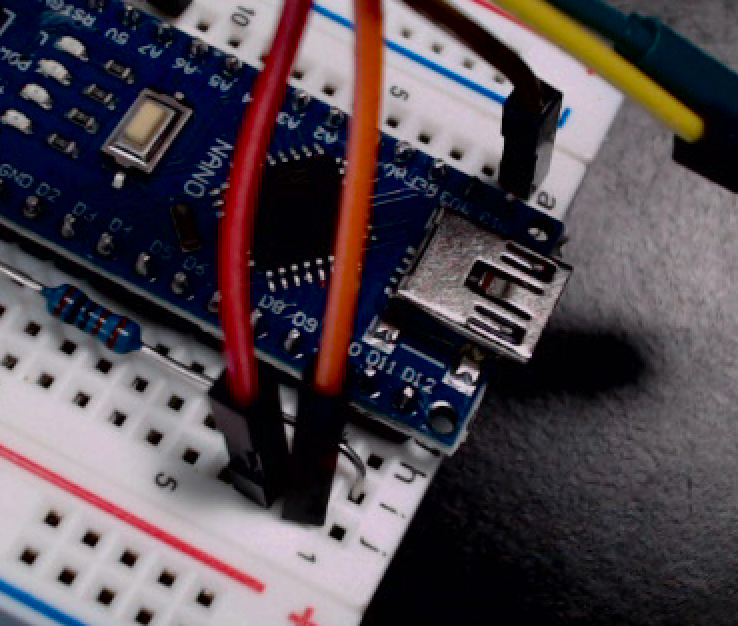
\includegraphics[width=0.27\textwidth]{display-module-DIN}
        \label{fig:display-module-DIN}
    }
    \hfil
    \subfloat[The display module will be powered by the breadboard's power
        bus] {
        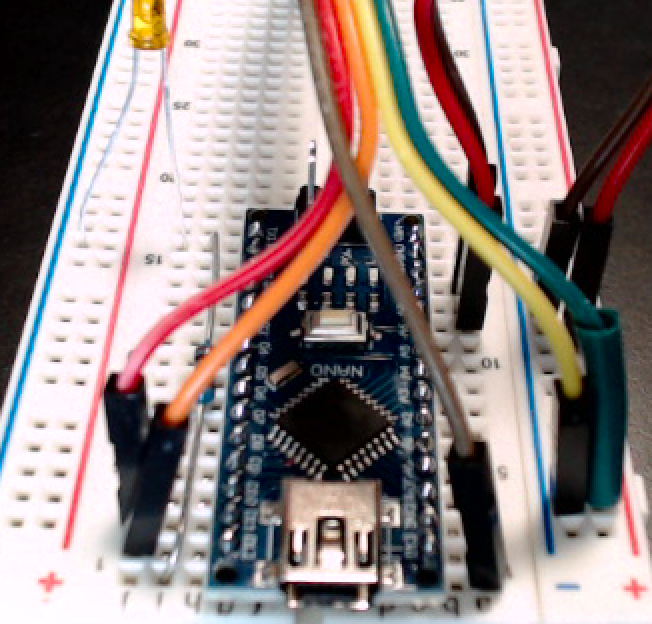
\includegraphics[width=0.27\textwidth]{display-module-power}
        \label{fig:display-module-power}
    }
    \caption{Connecting the Display Module.}
\end{figure}

When you have finished connecting the display module, there should be the
electrical connections described in Table~\ref{tab:display}.

\begin{table}
    \begin{center}\begin{tabular}{||c|c|c||} \hline\hline
    Display Module Pin  & \nano\ pin    & Pulled High/Low \\ \hline
    \texttt{CLK}         & \texttt{D13}  & \\
    \texttt{CS}          & \texttt{D10}  & \\
    \texttt{DIN}         & \texttt{D11}  & \\
    \texttt{GND}         &               & Pulled Low \\
    \texttt{VCC}         &               & Pulled High \\ \hline\hline
    \end{tabular}\end{center}
    \caption{Electrical Connections for External LED.\label{tab:display}}
\end{table}

\checkpoint{connected the display module to the breadboard}

In the Arduino IDE, open \textit{DisplayTest.ino}. Connect your \nano\ to the
computer. Compile \textit{DisplayTest.ino} and upload it to your \nano. You
should see {\dviiseg 8.} move back and forth across the display
(Figure~\ref{fig:display-test}). You may be able to see the \nano's built-in
LED blink rapidly: recall that it's connected to pin 13, which is used as the
clock signal when the \nano\ sends data to the display module.

\begin{figure}
    \centering
    \animategraphics[autoplay,palindrome,height=5cm]{10}{animations/displaytest-}{0}{7}
    \caption{\textit{DisplayTest.ino} illuminates all segments on a digit, one
        digit at a time.\label{fig:display-test}}
\end{figure}

\section{Input Devices}

\subsection{NAND Gates}\label{sec:nand}

The 74LS20 ``chip'' is an integrated circuit (IC) that holds two 4-input NAND
gates. It is in a \textit{dual inline package} (DIP), and solderless
breadboards are designed for the DIP form factor to straddle the breadboard's
center divider. A notch on the left side of the DIP helps us orient the IC; the
pins are numbered counter-clockwise from the lower-left to the upper-left
(Figure~\ref{fig:nand-annotated}). The relationship between the 74LS20's pins
and the NAND gates' inputs and outputs is shown in
Figure~\ref{fig:nand-pinout}.

Figure~\ref{fig:nand-diagram} shows the wiring to install the 74LS20.

\begin{figure}
    \centering
    \subfloat[Pin numbers for the 74LS20.]{
        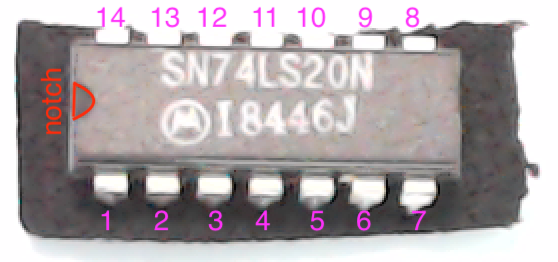
\includegraphics[width=6cm]{nand-annotated}
        \label{fig:nand-annotated}
    }
    \hfil
    \subfloat[Connection diagram showing the 74LS20's pinout.]{
        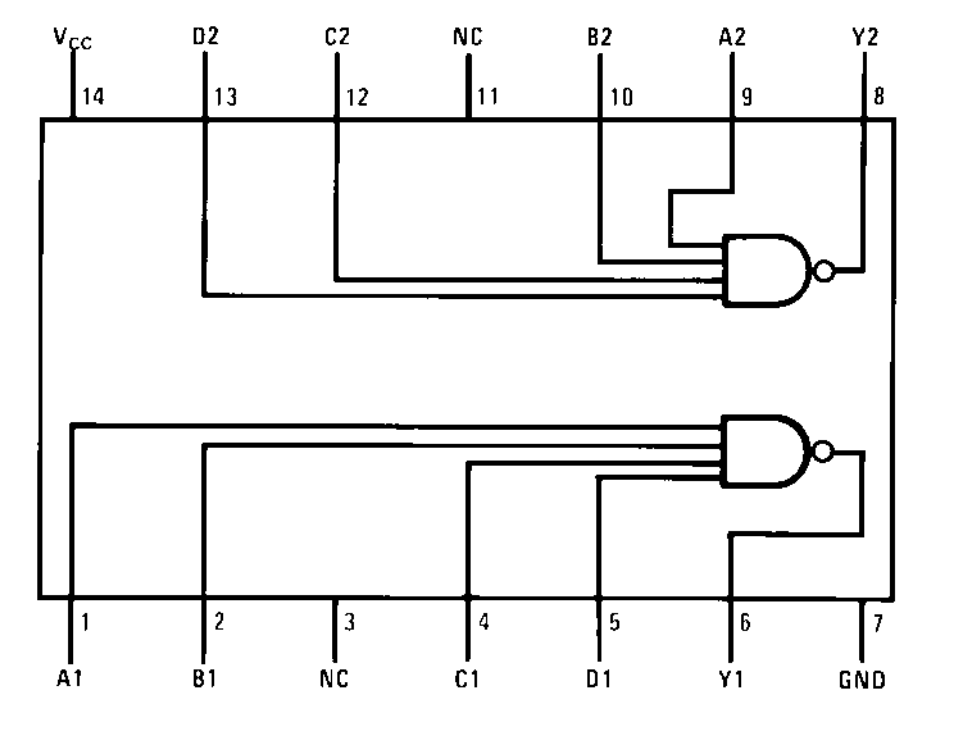
\includegraphics[width=6cm]{nand-pinout}
        \label{fig:nand-pinout}
    }
    \caption{Pin information for the 74LS20.}
\end{figure}

\begin{figure}
    \centering
    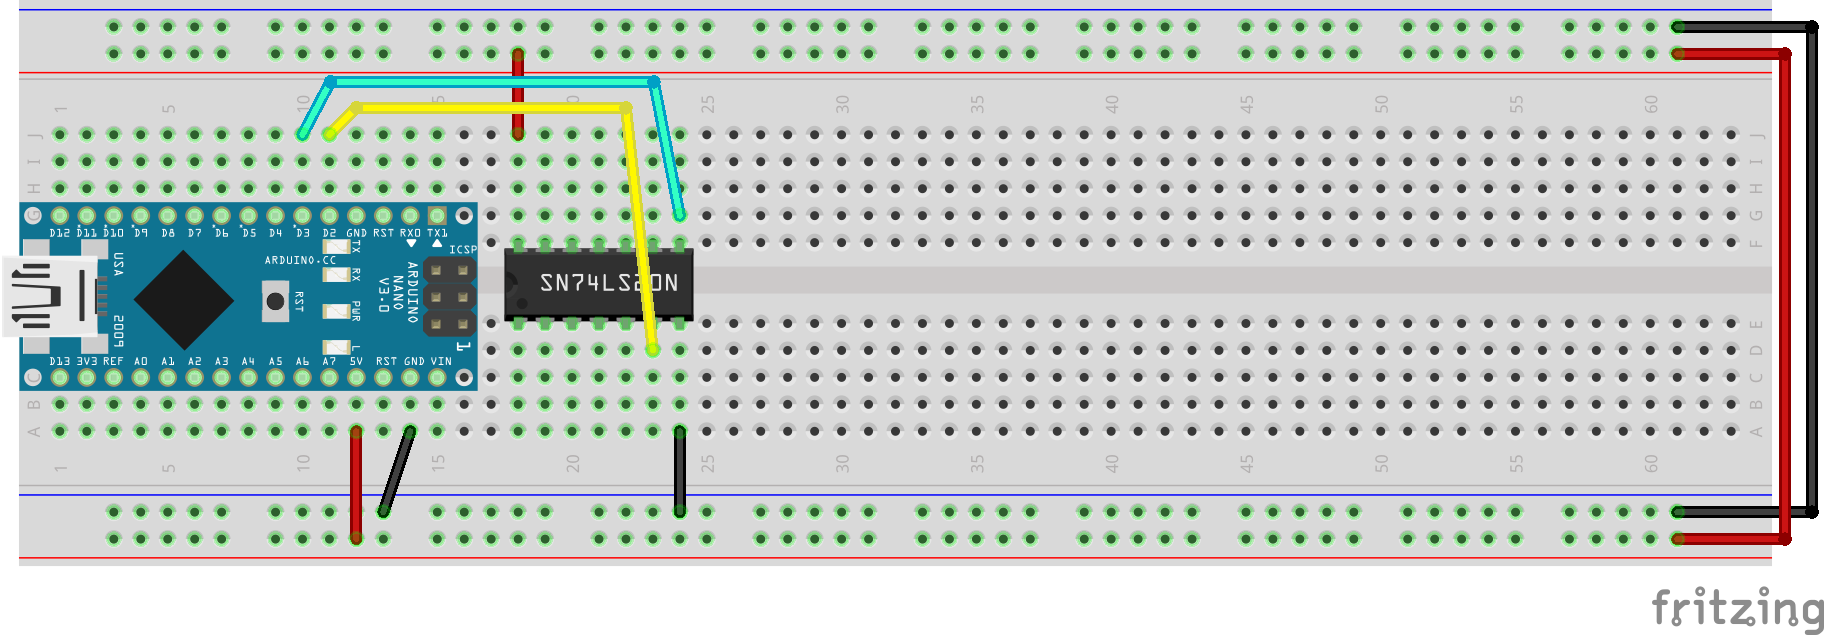
\includegraphics[width=0.9\textwidth]{fritzing_images/nand}
    \caption{Diagram of the 74LS20's installation.
        \label{fig:nand-diagram}}
\end{figure}

\disconnect\

Remove the anti-static foam from the 74LS20's pins. As described in the
\href{https://learn.adafruit.com/breadboards-for-beginners/breadboard-usage}{guide
at adafruit.com}, gently press the 74LS20's pins against a tabletop until
they're approximately square to the IC's case. With the its notch to the left,
place the 74LS20 on the breadboard straddling the center divider on rows 18-24.
Double-check that the 74LS20's pins 1-7 are on contact points e18-e24 and that
pins 8-14 are on contact points f24-f18 (Figure~\ref{fig:nand-ready} shows that
the IC's pins are not splayed outside the contact points nor are folded under
the IC's case). Gently press on the 74LS20 to insert the pins into the contact
points, using a slight rocking motion if necessary. As shown in
Figure~\ref{fig:nand-inserted}, the IC is fully inserted when its case is flush
with the breadboard.

\begin{figure}
    \centering
    \subfloat[Integrated circuit ready to be inserted.]{
        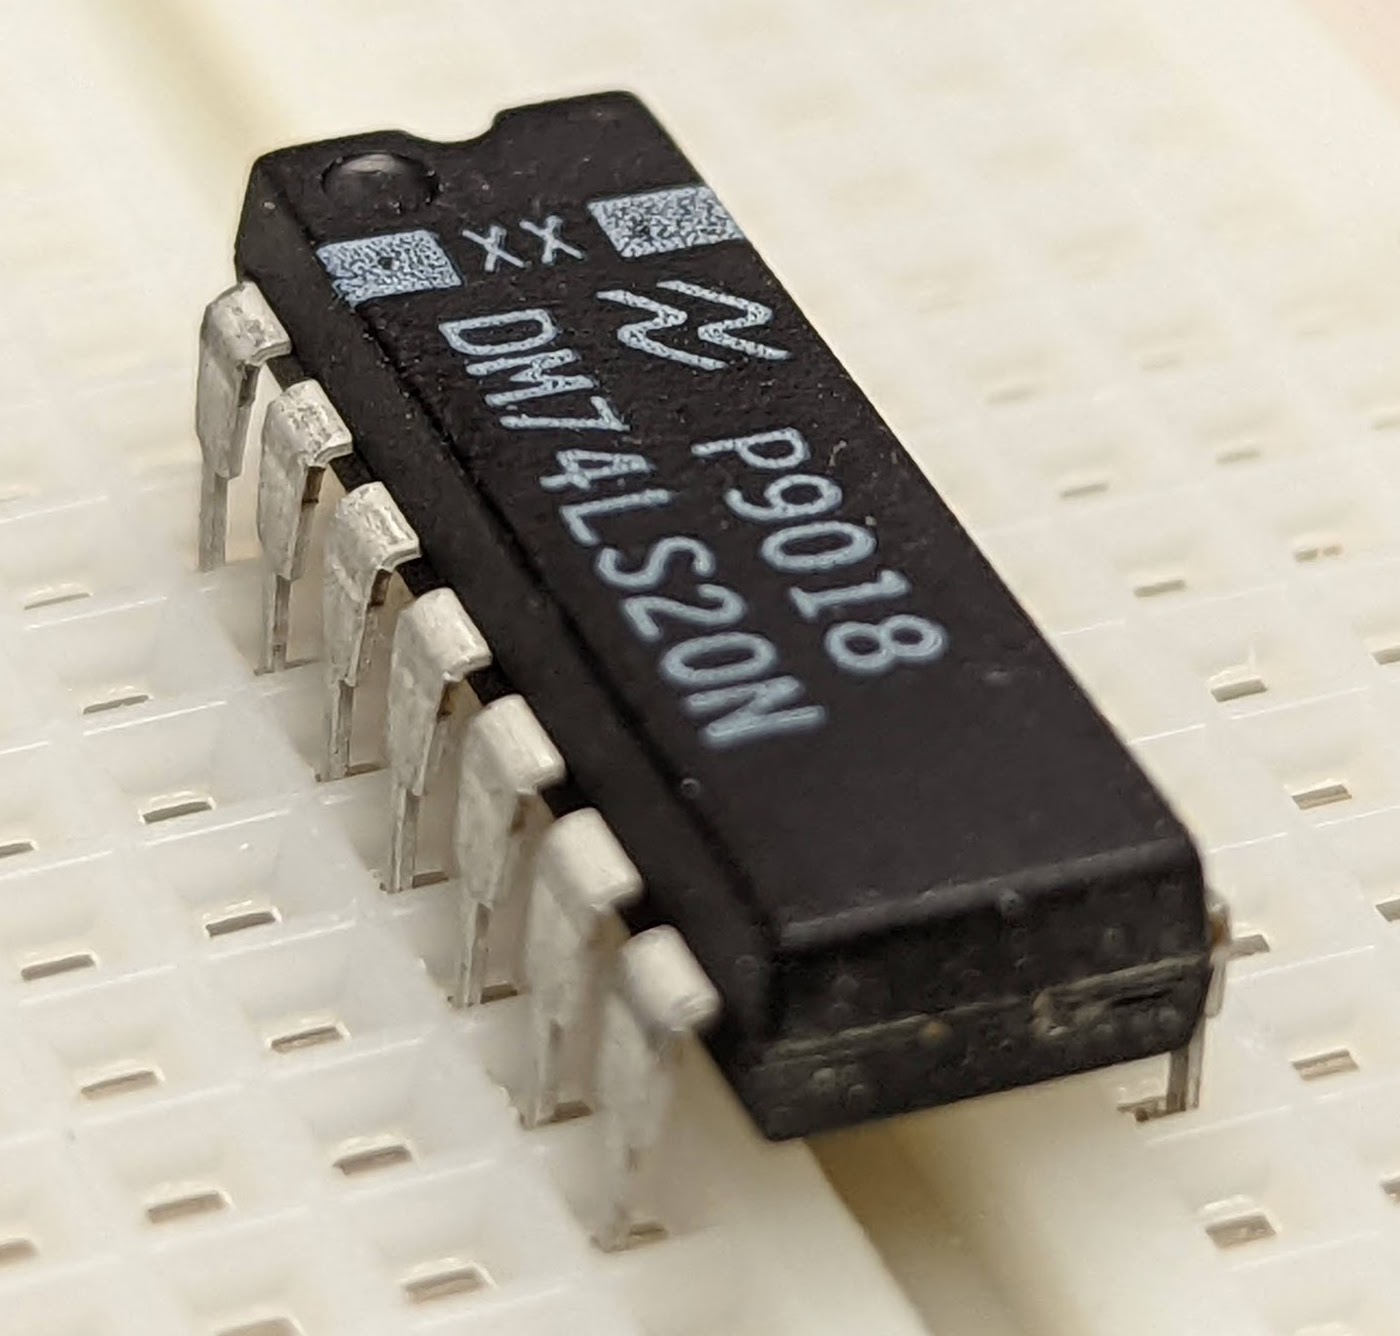
\includegraphics[height=4cm]{nand-ready-to-insert}
        \label{fig:nand-ready}
    }
    \hfil
    \subfloat[Integrated circuit fully inserted.]{
        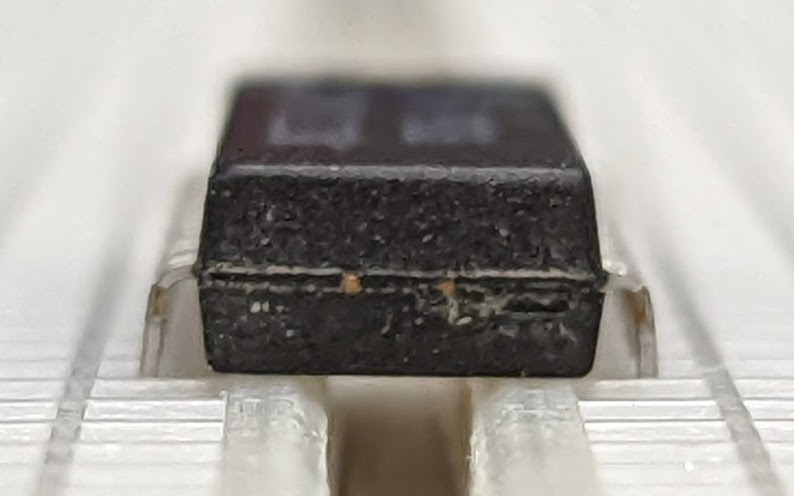
\includegraphics[height=4cm]{nand-fully-inserted}
        \label{fig:nand-inserted}
    }
    \caption{Inserting the 74LS20.}
\end{figure}

Peel one wire from the \rainbow; use this wire to connect contact point j18
(electrically connected to the 74LS20's $\mathtt{V_{CC}}$, pin 14) to a \power.
Peel off another wire from the \rainbow; use this wire to connect contact point
a24 (electrically connected to the 74LS20's \texttt{GND}, pin 7) to a \ground.
See Figure~\ref{fig:nand-power}.

Peel a two-wire cable from the \rainbow. Use this cable to connect contact
point d23 (electrically connected to the 74LS20's \texttt{Y1}, pin 6) to
contact point j11 (electrically connected to the \nano's \texttt{D2} pin), and
to connect contact point g24 (electrically connected to the 74LS20's
\texttt{Y2}, pin 8) to contact point j10 (electrically connected to the
\nano's \texttt{D3} pin). See Figure~\ref{fig:nand-outputs}.

\begin{figure}
    \centering
    \subfloat[The 74LS20 connected to power and ground.]{
        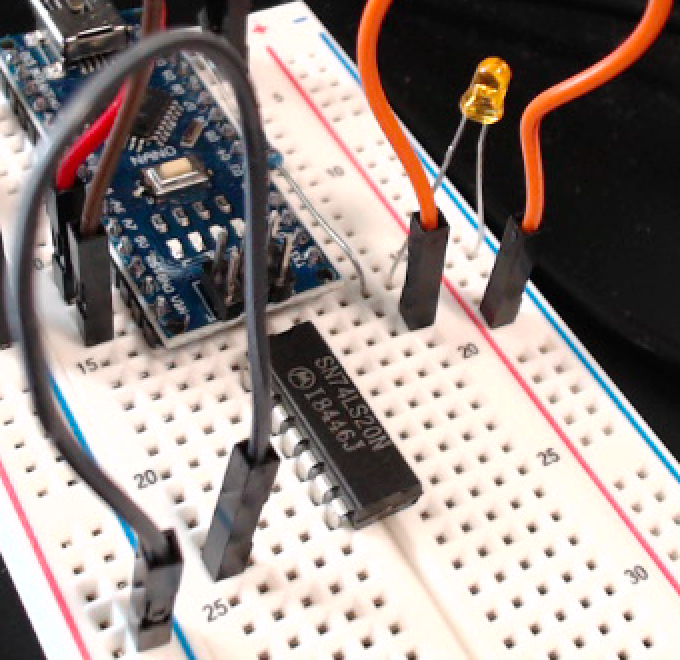
\includegraphics[width=.4\textwidth]{nand-power}
        \label{fig:nand-power}
    }
    \hfil
    \subfloat[The 74LS20's outputs connected to the \nano.]{
        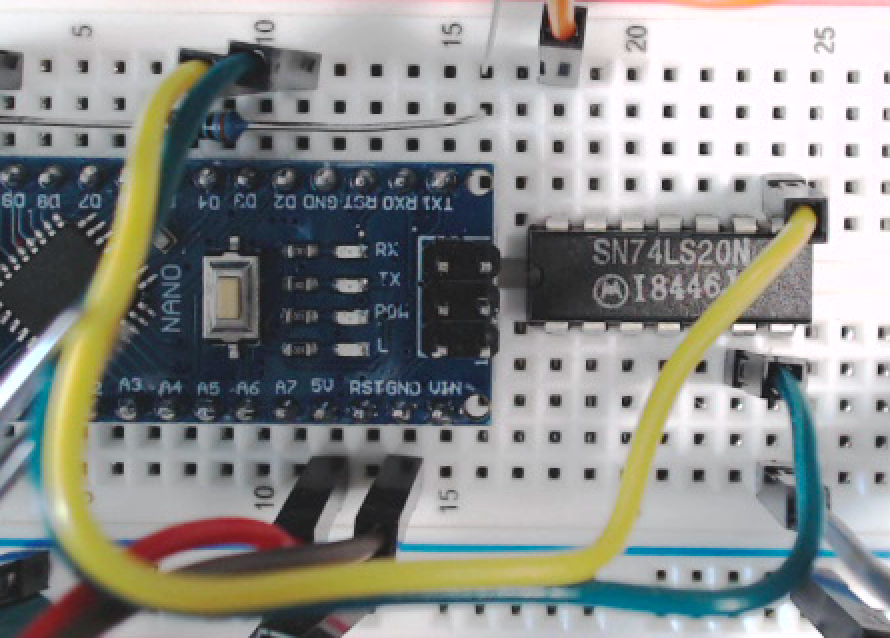
\includegraphics[width=.5\textwidth]{nand-outputs}
        \label{fig:nand-outputs}
    }
    \caption{Wiring the 74LS20.}
\end{figure}

When you have finished wiring the 74LS20, there should be the
electrical connections described in Table~\ref{tab:nand}.

\begin{table}
    \begin{center}\begin{tabular}{||c|c|c||} \hline\hline
    74LS20 Pin  & \nano\ pin    & Pulled High/Low \\ \hline
    6           & \texttt{D2}   & \\
    7           &               & Pulled Low \\
    8           & \texttt{D3}   & \\
    14          &               & Pulled High \\ \hline\hline
    \end{tabular}\end{center}
    \caption{Initial Electrical Connections for NAND Gates.\label{tab:nand}}
\end{table}

\checkpoint{inserted and wired the 74LS20}

\newpage

\subsection{Matrix Keypad}

\begin{wrapfigure}{r}{0.3\textwidth}
    \centering
    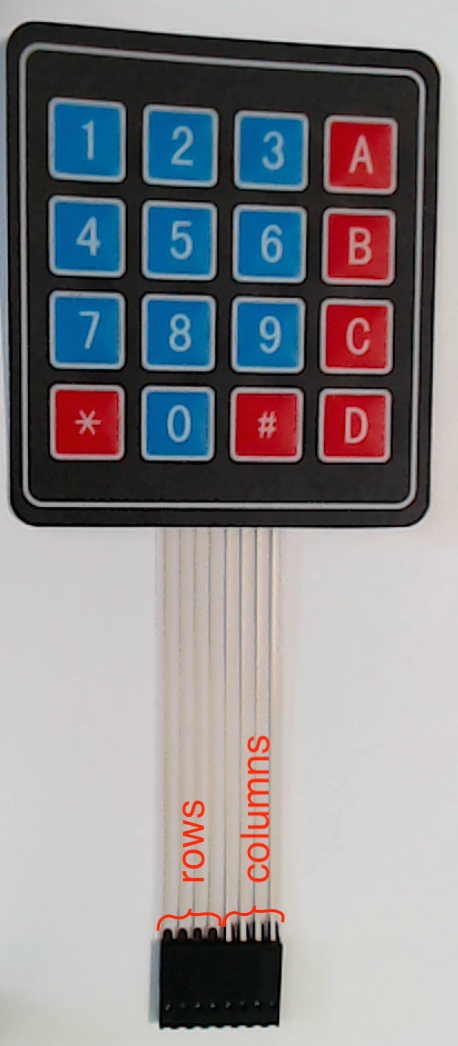
\includegraphics[width=0.25\textwidth]{keypad-annotated}
    \caption{The numeric keypad's header has four row pins and four column pins.\label{fig:keypad-annotated}}
\end{wrapfigure}

Observe that the matrix keypad has sixteen buttons has eight pins in its female
connector. As shown in Figure~\ref{fig:keypad-annotated}, when the keypad is
face-up and oriented for reading, the four pins on the left are the
\textit{row} pins, and the four pins on the right are the \textit{column} pins.
From left-to-right, we will name these pins \texttt{row1}, \texttt{row4},
\texttt{row7}, \texttt{row*}, \texttt{column1}, \texttt{column2},
\texttt{column3}, \texttt{columnA}

Figure~\ref{fig:keypad-diagram} shows a diagram of of the wiring for the
matrix keypad.

\begin{figure}[p]
    \centering
    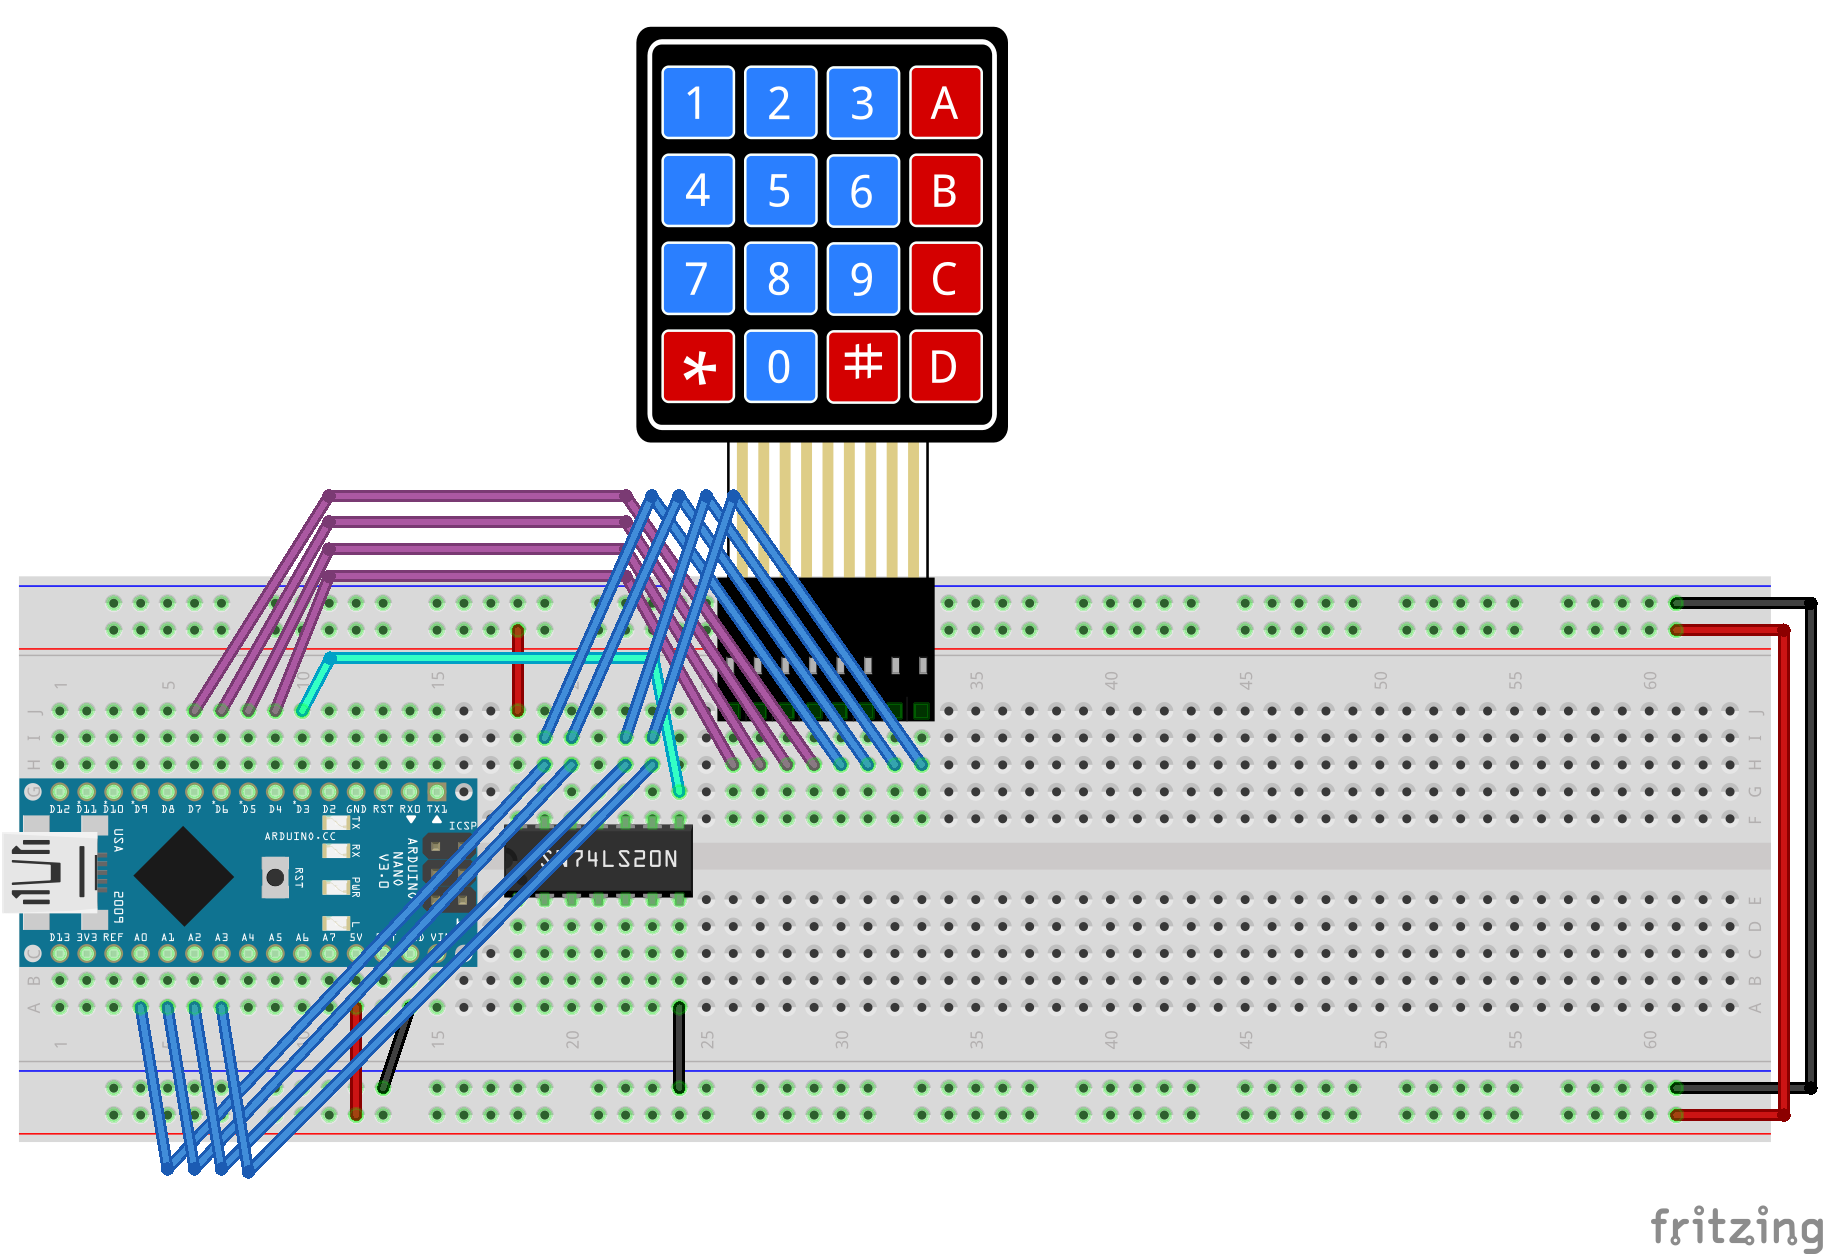
\includegraphics[width=0.9\textwidth]{fritzing_images/keypad}
    \caption{Diagram of wiring associated with matrix keyboard input.
        \textit{Note: connection between the 74LS20's pin 8 and the \nano's
        \texttt{D3} pin was previously installed in Section~\ref{sec:nand}.}
        \label{fig:keypad-diagram}}
\end{figure}

If your 8-pin male-male header strip is not already inserted into the keypad's
female connectors, insert it into the female connectors now. If your male-male
header strip has more than eight pins, position the excess pins to the right of
the column pins. Connect your keypad to your breadboard such that \texttt{row1}
is in contact point j26, and \texttt{columnA} is in contact point j33 (and any
unused pins on the male-male header are in contact points j34, j35, etc.); see
Figure~\ref{fig:keypad-header}.

Peel off a 4-conductor cable from the \rainbow. Insert one end in contact
points h26-h29, in the same breadboard rows as the keypad's row pins
(Figure~\ref{fig:keypad-row-cable}). Insert the other end of the cable in
contact points j9-j6 (Figure~\ref{fig:keypad-row-nano}). You want the \nano's
\texttt{D4} pin to connect to the keypad's \texttt{row1} pin, \texttt{D5} to
\texttt{row4}, \texttt{D6} to \texttt{row7}, and \texttt{D7} to \texttt{row*}
(Figure~\ref{fig:keypad-row-full}).

Peel off another 4-conductor cable from the \rainbow. Insert one end in contact
points h30-h33, in the same breadboard rows as the keypad's column pins. Insert
the other end of the cable in contact points i19, i20, i22, and i23
(electrically connected to the 74LS20's \texttt{D2}, \texttt{C2}, \texttt{B2},
and \texttt{A2}: pins 13, 12, 10, and 9). See
Figure~\ref{fig:keypad-col-nand}. Peel off another 4-conductor cable from
the \rainbow. Insert one end in contact points h19, h20, h22, and h23. Insert
the other end in contact points a4-a7 (electrically connected to the \nano's
\texttt{A0}-\texttt{A3} pins). See Figure~\ref{fig:keypad-col-nano}.

\begin{figure}
    \centering
    \subfloat[The matrix keypad's connector, with the male-male header strip,
        just before being inserted into the breadboard. Note the excess header
        strip's excess pin to the right of the column pins, in contact point
        j34.]{
        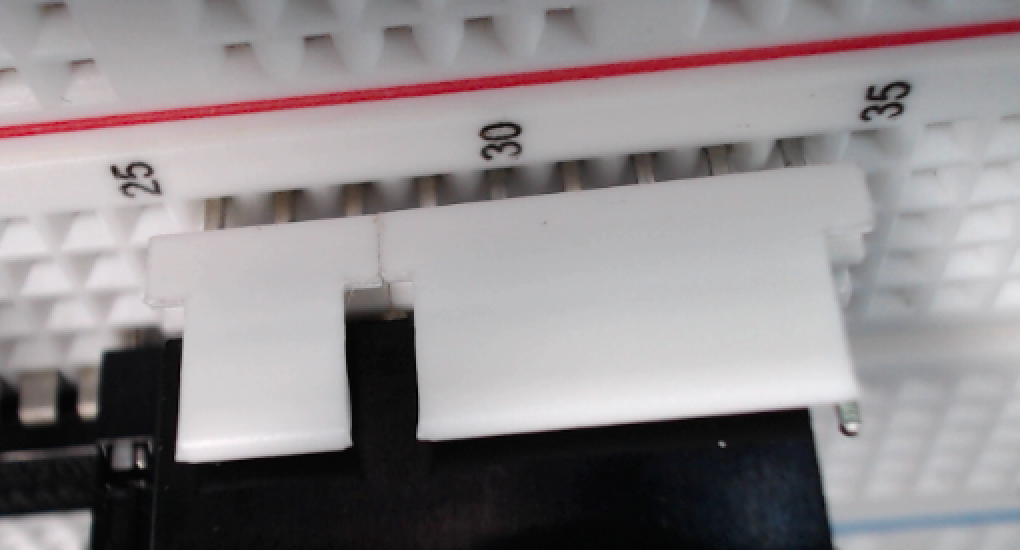
\includegraphics[width=.5\textwidth]{keypad-header}
        \label{fig:keypad-header}
    }
    \hfil
    \subfloat[One end of the ``rows'' cable electrically connected to the
        keypad's row pins.]{
        \includegraphics[width=.4\textwidth]{keypad-row-cable}
        \label{fig:keypad-row-cable}
    }

    \subfloat[The other end of the ``rows'' cable electrically connected to the \nano's \texttt{D4}-\texttt{D7} pins.]{
        \includegraphics[width=.4\textwidth]{keypad-row-nano}
        \label{fig:keypad-row-nano}
    }
    \hfil
    \subfloat[Connection between the keypad's row pins and the \nano's
        \texttt{D4}-\texttt{D7} pins.]{
        \includegraphics[width=.5\textwidth]{keypad-row-full}
        \label{fig:keypad-row-full}
    }

    \subfloat[Connection between the keypad's column pins and the 74LS20.]{
        \includegraphics[width=.4\textwidth]{keypad-col-nand}
        \label{fig:keypad-col-nand}
    }
    \hfil
    \subfloat[Connection between the the 74LS20 and the \nano's \texttt{A0}-\texttt{A3} pins.]{
        \includegraphics[width=.5\textwidth]{keypad-col-nano}
        \label{fig:keypad-col-nano}
    }
    \caption{Wiring the Matrix Keypad.}
\end{figure}

When you have finished setting up the keypad wiring, there should be the
electrical paths described in Table~\ref{tab:keypad}.

\begin{table}
    \begin{center}\begin{tabular}{||c|c|c||} \hline\hline
    Keypad pin          & 74LS20            & \nano\ pin \\ \hline
    \texttt{row1}       &                   & \texttt{D4} \\
    \texttt{row4}       &                   & \texttt{D5} \\
    \texttt{row7}       &                   & \texttt{D6} \\
    \texttt{row*}       &                   & \texttt{D7} \\
    \texttt{column1}    & Upper NAND Input  & \texttt{A0} \\
    \texttt{column2}    & Upper NAND Input  & \texttt{A1} \\
    \texttt{column3}    & Upper NAND Input  & \texttt{A2} \\
    \texttt{columnA}    & Upper NAND Input  & \texttt{A3} \\
                        & Upper NAND Output & \texttt{D3} \\ \hline\hline
    \end{tabular}\end{center}
    \caption{Electrical Paths for Matrix Keypad.\label{tab:keypad}}
\end{table}

\checkpoint{inserted and wired the matrix keypad}

In the Arduino IDE, open \textit{InputTest.ino}. Connect your \nano\ to the
computer. Compile \textit{InputTest.ino} and upload it to your \nano. Open the
IDE's Serial Monitor (\textit{Tools} $\rightarrow$ \textit{Serial Monitor}).
You will see several lines reporting the current value of various inputs. (You
will also see the \nano's \texttt{TX} LED blinking as the \nano\ sends these
lines to your computer.) Right now, KEYPAD~COLUMNS is always 1111, and
KEYPAD~NAND is always 0. Notice that when you press 1, 4, 7, or *,
KEYPAD~COLUMNS becomes 0111; similarly, pressing a button in the 2$^{nd}$
column causes KEYPAD~COLUMNS to become 1011; in the 3$^{rd}$ column, 1101; and
in the A$^{th}$ column, 1110. Whenever any keypad button is pressed,
KEYPAD~NAND becomes 1. Be sure to test all 16 keys.

\subsection{Slider Switches}

In this section, you will install the ``slider'' switches that toggle between
their two positions, holding their position until toggled again. We will wire
them such that when a switch is toggled to the left, it will produce a 0, and
when it is toggled to the right, it will produce a 1.
Figure~\ref{fig:switch-diagram} shows a diagram of of the wiring for the
slider switches.

\begin{figure}[p]
    \centering
    \includegraphics[width=0.9\textwidth]{fritzing_images/switch}
    \caption{Diagram of wiring associated with toggle switch input.
        \label{fig:switch-diagram}}
\end{figure}

\disconnect\

Insert one slider switch into contact points a29-a31. Peel off one wire from
the \rainbow, and use it to connect contact point e29 to the upper \ground.
Place the other slider switch into contact points a34-a36. Peel off another
wire from the \rainbow, and use it to connect contact point e34 to the upper
\ground. % See Figure~\ref{fig:switch-power-ground}.

Peel off one wire from the \rainbow, and use it to connect contact point d30
(electrically connected to the left switch's center pin) to contact point a8
(electrically connected to the \nano's \texttt{A4} pin). Peel off another wire
from the \rainbow, and use it to connect contact point d35 (electrically
connected to the right switch's center pin) to contact point a9 (electrically
connected to the \nano's \texttt{A5} pin). % See Figure~\ref{fig:switch-nano}.
See Figure~\ref{fig:switch-spst}.

The switches' right pins will not be electrically connected to anything.

% \begin{figure}
%     \centering
%     \subfloat[The slider switches, each with their left pin grounded and their
%         right pin connected to 5V.]{
%         \includegraphics[width=0.3\textwidth]{switch-power-ground}
%         \label{fig:switch-power-ground}
%     }
%     \hfil
%     \subfloat[Connections between the \nano\ and the slider switches.]{
%         \includegraphics[width=0.6\textwidth]{switch-nano}
%         \label{fig:switch-nano}
%     }
%     \caption{Wiring the Slider Switches}
% \end{figure}

\begin{figure}
    \centering
    \includegraphics[width=0.6\textwidth]{switch-spst}
    \caption{The slider switches, each with one pin grounded, one pin connected
        to the \nano, and one pin floating. \label{fig:switch-spst}}
\end{figure}

When you have finished setting up the switches' wiring, there should be the
electrical connections described in Table~\ref{tab:switch}.

\begin{table}
    \begin{center}\begin{tabular}{||c|c|c||} \hline\hline
    Switch                      & \nano\ pin    & Pulled High/Low \\ \hline
    Left switch's left pin      &               & Pulled Low \\
    Left switch's center pin    & \texttt{A4}   & \\
    Left switch's right pin     & \multicolumn{2}{c||}{not connected / floating} \\
    Right switch's left pin     &               & Pulled Low \\
    Right switch's center pin   & \texttt{A5}   & \\
    Right switch's right pin    & \multicolumn{2}{c||}{not connected / floating} \\ \hline\hline
    \end{tabular}\end{center}
    \caption{Electrical Connections for Slider Switches.\label{tab:switch}}
\end{table}

\checkpoint{inserted and wired the slider switches}

Connect your \nano\ to the computer. In the IDE's Serial Monitor, notice that
the LEFT~SWITCH is 0 when the left switch is toggled to the left, and it is 1
when the left switch is toggled to the right. Similarly, the RIGHT~SWITCH's
value is 0 or 1, depending on whether the right switch is toggled to the left
or right.

\subsection{Momentary Pushbuttons}

If your momentary pushbuttons are attached to a cardboard strip with tape,
remove them from the cardboard strip. If your momentary pushbuttons' leads have
metal tabs at the end (Figure~\ref{fig:pushbutton-tabs}), you will need to
snip off the tabs before inserting the pushbutton leads into the breadboard;
ordinary scissors will suffice for this task. Regardless of whether the leads
have metal tabs at the end, you may optionally trim the leads to be about
$\frac{1}{4}$in (6.4mm) long -- you can use the exposed lead from a jumper wire
as a reference -- so that the pushbuttons sit flush on the breadboard. It is
not necessary that they sit flush; this is simply to keep the buttons from
wiggling under your fingers. \textit{Do not cut the leads shorter than
$\mathit{\frac{1}{8}}$in (3.2mm)!} \textbf{Be sure to use eye protection in
case the leads' ends fly off when you snip them.}

These are ``normally open'' momentary ``switches'' that close when pressed and
re-open when released. We will wire the pushbuttons such that they normally
produce a 1, and when pressed will produce a 0.
Figure~\ref{fig:pushbutton-diagram} shows a diagram of of the wiring for the
pushbuttons.

\begin{figure}
    \centering
    \includegraphics[height=2cm]{pushbutton-tabs}
    \caption{Some momentary pushbuttons have metal tabs on their leads.\label{fig:pushbutton-tabs}}
\end{figure}

\begin{figure}
    \centering
    \includegraphics[width=0.9\textwidth]{fritzing_images/pushbutton}
    \caption{Diagram of wiring associated with momentary pushbutton input.
        \textit{Note: connection between the 74LS20's pin 6 and the \nano's
        \texttt{D2} pin was previously installed in Section~\ref{sec:nand}.}
        \label{fig:pushbutton-diagram}}
\end{figure}

\disconnect\

Insert the leads of one pushbutton into contact points a39 and a41. Peel off
one wire from the \rainbow, and use it to connect contact point e41 to the
upper \ground. Insert the leads of the other pushbutton into contact points a43
and a45. Peel off one wire from the \rainbow, and use it to connect contact
point e45 to the upper \ground. See Figure~\ref{fig:pushbutton-grounded}.

Peel off a 2-conductor cable from the \rainbow, and use it to connect contact
points a21 and a22 (electrically connected to the 74LS20's \texttt{C1} and
\texttt{D1}, pins 4 and 5) to a \power. Peel off another 2-conductor cable and
use it to connect contact points d39 and d43 (electrically connected to the
ungrounded sides of the pushbuttons) to the 74LS20: contact point d39 should be
connected to contact point b19 (electrically connected to the 74LS20's
\texttt{B1}, pin 2), and contact point d43 should be connected to contact point
b18 (electrically connected to the 74LS20's \texttt{A1}, pin 1). See
Figure~\ref{fig:pushbutton-nand}.

Peel off another 2-conductor cable from the \rainbow, and use it to connect
contact points j4 and j5 (electrically connected to the \nano's \texttt{D9} and
\texttt{D8} pins) to contact points c18 and c19 (electrically connected to the
74LS20's \texttt{A1} and \texttt{B1}, and to the pushbuttons through the cable
you installed in the previous paragraph), respectively. See
Figure~\ref{fig:pushbutton-nano}.

\begin{figure}\begin{multicols}{2}
    \centering
    \subfloat[The momentary pushbuttons, each with one lead grounded.]{
        \includegraphics[width=0.4\textwidth]{pushbutton-grounded}
        \label{fig:pushbutton-grounded}
    }
    \columnbreak

    \subfloat[Connections between the momentary pushbuttons and the 74LS20.]{
        \includegraphics[width=0.55\textwidth]{pushbutton-nand}
        \label{fig:pushbutton-nand}
    }

    \subfloat[Connections between the \nano\ and wiring to the momentary
        pushbuttons.]{
        \includegraphics[width=.55\textwidth]{pushbutton-nano}
        \label{fig:pushbutton-nano}
    }
    \end{multicols}
    \caption{Wiring the Momentary Pushbuttons.}
\end{figure}

When you have finished setting up the pushbuttons' wiring, there should be the
electrical paths described in Table~\ref{tab:pushbutton}.

\begin{table}
    \begin{center}\begin{tabular}{||c|c|c|c||} \hline\hline
    Pushbutton                      & 74LS20            & \nano\ pin    & Pulled High/Low \\ \hline
    Left button's grounded lead     &                   &               & Pulled Low \\
    Left button's ungrounded lead   & Lower NAND Input  & \texttt{D8}   & \\
    Right button's grounded lead    &                   &               & Pulled Low \\
    Right button's ungrounded lead  & Lower NAND Input  & \texttt{D9}   & \\
                                    & Lower NAND Input  &               & Pulled High \\
                                    & Lower NAND Input  &               & Pulled High \\
                                    & Lower NAND Output & \texttt{D2}   & \\ \hline\hline
    \end{tabular}\end{center}
    \caption{Electrical Paths for Momentary Pushbuttons.\label{tab:pushbutton}}
\end{table}

\checkpoint{inserted and wired the momentary pushbuttons}

Connect your \nano\ to the computer. In the IDE's Serial Monitor, notice that
the LEFT~BUTTON is always 1, the RIGHT~BUTTON is always 1, and the BUTTON~NAND
is always 0. Notice that when you press a button, the Serial Monitor shows that
its value becomes 0, and when you release a button, its value becomes 1 again.
If either button is pressed, BUTTON~NAND becomes 1, and it is 0 only when both
buttons are not pressed.

\section*{Kit Assembly is Complete}

You have now finished assembling the class kit (Figure~\ref{fig:complete}). In
the upcoming I/O labs, you will use the kit to learn about memory-mapped I/O
and about handling low-level interrupts.

\begin{figure}
    \centering
    \subfloat[]{
        \includegraphics[height=0.55\textheight]{fritzing_images/complete}
        \label{fig:complete-diagram}
    }

    \subfloat[]{
        \includegraphics[height=0.35\textheight]{completed-kit}
        \label{fig:complete-kit}
    }
    \caption{The fully-assembled class kit.\label{fig:complete}}
\end{figure}

\section*{Turn-in and Grading}

When you have completed this assignment, upload \textit{checkpoints.txt} to
\filesubmission.

This assignment is worth 1 point, with up to 5 bonus points for helping other
students. \\

Rubric:
\begin{description}
\rubricitem{0.5}{You bring your fully-assembled class kit to your lab section
    the week it is due.}
\rubricitem{0.5}{You upload the completed \textit{checkpoints.txt} file to
    \filesubmission.}
\bonusitem{0.1}{For each checkpoint you verify for fellow students, as
    reported in their \textit{checkpoints.txt} files; maximum of 5.0 bonus
    points.}
\end{description}

\end{document}
